\documentclass[journal]{IEEEtran}

% Packages
\usepackage[T1]{fontenc}
\usepackage{amsmath,amssymb,amsfonts}
\usepackage{booktabs}
\usepackage{graphicx}
\usepackage{multirow}
\usepackage{array}
\usepackage{url}
\usepackage{xcolor}
\usepackage{balance}

% Custom commands
\newcommand{\E}{\mathcal{E}}               % Economic decision space
\DeclareMathOperator*{\argmin}{arg\,min}

\begin{document}

\title{Geometric Prediction of Economic Behavior:\\Cross-Domain Validation Across Game Theory\\and Prospect Theory}

\author{Andrew~H.~Bond,~\IEEEmembership{Senior Member,~IEEE}%
\thanks{A.~H.~Bond is with the Department of Computer Engineering, San Jos\'{e} State University, San Jos\'{e}, CA 95192 USA (e-mail: andrew.bond@sjsu.edu; ORCID: 0009-0003-2599-6158).}%
\thanks{Manuscript received March 26, 2026; revised June 10, 2026; accepted September 6, 2026.}}

\markboth{IEEE Transactions on Computational Social Systems}%
{Bond: Geometric Prediction of Economic Behavior}

\maketitle

\begin{abstract}
We study a geometric model of economic decision-making in which each alternative is encoded as a point in a nine-dimensional decision space and the cost of moving from a task-specific reference point to that alternative is a Mahalanobis distance under a diagonal covariance matrix.
Three covariance variances are fitted on nine bargaining and public-goods targets by an exhaustive search over active dimensions.
The same variances are then applied, without refitting, to six classic prospect-theory choice problems and one historical ultimatum replication.
The active-set structure was selected using the complete benchmark, so the lottery results demonstrate cross-domain parameter reuse within a jointly selected architecture rather than fully out-of-sample prediction.
The selected model activates social impact, virtue and identity, and epistemic status.
It matches all sixteen aggregate targets within stated tolerances with a mean absolute error of 2.70 percentage points.
The monetary dimension is inactive, which the model expresses as a falsifiable corollary that multiplying every stake by a constant leaves predicted offers and rejections unchanged.
We test that corollary on the high-stakes ultimatum data of Andersen and co-authors from Meghalaya in northeast India, with 458 responders and stakes from 20 to 20,000 rupees, the largest exceeding the average yearly income of the participants.
Three pre-specified tests reject the calibrated model's stake-scaling invariance, which shows that the share-normalized encoding and the selected metric do not extend unchanged to consequential-stake settings.
The result motivates, but does not test, a monetary coordinate in absolute or income units with finite sensitivity.
The paper specifies every encoding rule, search step, and fitted or coded constant of the reference implementation, states which targets entered each fitting and selection step, reports uncertainty where individual-level data are recoverable, and presents the contribution as a falsifiable cross-domain modeling architecture rather than a unification of game theory and prospect theory.
\end{abstract}

\begin{IEEEkeywords}
Computational social systems, geometric economics, behavioral prediction, game theory, prospect theory, Mahalanobis distance, bounded rationality, cross-domain validation, structural fuzzing.
\end{IEEEkeywords}


%==============================================================================
\section{Introduction}
\label{sec:intro}
%==============================================================================

\IEEEPARstart{P}{redicting} economic behavior is a central problem for computational social systems because social platforms, markets, energy systems, and policy mechanisms all depend on agents whose choices are neither purely monetary nor fully random.
Expected-utility theory, axiomatized by von~Neumann and Morgenstern~\cite{vonneumann1944} and extended by Savage~\cite{savage1954}, provides a clean scalar account of choice under risk.
Behavioral economics has shown that actual choices also reflect reference dependence, loss aversion, probability weighting, fairness, reciprocity, and social meaning~\cite{kahneman1979,tversky1992,fehr1999,bolton2000}.
Large replications show that many prospect-theory patterns are robust across countries while also exhibiting meaningful heterogeneity~\cite{ruggeri2020,henrich2010}.

Existing models specialize by domain.
Cumulative Prospect Theory (CPT)~\cite{tversky1992} is powerful for risky lotteries but is not a model of strategic interaction.
Fehr--Schmidt inequality aversion~\cite{fehr1999} and ERC~\cite{bolton2000} address social preferences in games but do not model certainty effects, reflection effects, or probability weighting.
Computational game-theoretic models in socio-technical systems represent agents through payoffs, strategies, reinforcement rules, or negotiation protocols, but they still require a behavioral primitive that says which features of a situation are costly or attractive to the agent.

This paper asks whether such a primitive can be represented geometrically.
Each economic scenario is encoded as a task-specific reference point and a set of alternatives in a nine-dimensional decision space.
The dimensions describe monetary consequences, rights or entitlements, fairness, autonomy, privacy and trust, social impact, virtue and identity, legitimacy, and epistemic status.
A diagonal covariance matrix sets the cost of displacement along each dimension through a Mahalanobis distance.
For bargaining and public-goods games the prediction is the least costly offer or contribution.
For binary lottery choices a softmax rule maps the two costs to a population choice frequency.

The empirical design is deliberately modest.
We fit the covariance on nine game-theoretic targets and then apply the same covariance, without refitting the variances, to seven further targets, namely six classic prospect-theory problems and one historical ultimatum replication.
The benchmark asks whether a metric discovered from strategic interaction also organizes several canonical risky-choice phenomena.
It does not claim that the sixteen targets exhaust either literature or that the present encodings are uniquely correct.
Two constants of the choice rule and one reference coordinate of the historical target were themselves set from lottery and historical targets, and the active-set structure was ranked on all sixteen targets.
We say precisely which targets entered each step.

The selected model activates three dimensions, social impact, virtue and identity, and epistemic status.
Within the stated tolerances it matches all sixteen aggregate targets with a mean absolute error of 2.70 percentage points.
The monetary dimension is inactive in this calibration.
We treat that as a falsifiable context-specific finding rather than a universal claim, through a corollary the inactive dimension implies.
If money carries no cost, multiplying every stake by a constant must leave predicted offers and rejections unchanged.
We test the corollary on the high-stakes ultimatum data of Andersen and co-authors~\cite{andersen2011}, collected in Meghalaya in northeast India with stakes from 20 to 20,000 rupees.
All three pre-specified tests reject invariance.
The calibrated model predicts invariance, and that prediction fails, so the share-normalized encoding and the selected metric do not extend unchanged to stakes that exceed a year of income.
The result motivates, but does not test, a monetary coordinate in absolute or income units with finite sensitivity.

The paper makes six contributions.
It gives a self-contained geometric decision model whose encoding rules, metric, choice rules, temperature constants, structural search, and parameter accounting are all specified here and match the released reference implementation.
It reports a cross-domain benchmark in which a covariance fitted on game-theoretic targets is evaluated on prospect-theory and historical-replication targets without refitting the active variances, within an active-set structure selected on the full benchmark.
It identifies an interpretable active set, since exhaustive structural search selects social impact, identity, and epistemic status as the dominant metric dimensions in this benchmark.
It reports a direct empirical falsification of the calibrated model's stake-scaling invariance on individual-level high-stakes data, which demonstrates a failure of invariance without locating its boundary.
It separates the fitted metric parameters from the fixed encoding assumptions and reports targeted ablations of each.
It illustrates the use of the calibrated metric as a behavioral primitive in a minimal agent-based simulation and states the data needed for broader validation.

The remainder of the paper is organized as follows.
Section~\ref{sec:related} reviews related work.
Section~\ref{sec:framework} presents the geometric model.
Section~\ref{sec:encoding} gives the domain-specific encodings as implemented.
Section~\ref{sec:validation} describes the validation methodology.
Section~\ref{sec:results} presents results.
Section~\ref{sec:discussion} discusses implications and limitations.
Section~\ref{sec:conclusion} concludes.
%==============================================================================
\section{Related Work}
\label{sec:related}
%==============================================================================

\subsection{Prospect Theory and Cumulative Prospect Theory}

Kahneman and Tversky's original prospect theory~\cite{kahneman1979} introduced reference dependence, loss aversion, and probability weighting as descriptive corrections to expected-utility theory.
Cumulative Prospect Theory (CPT)~\cite{tversky1992} extended the model to continuous distributions and rank-dependent probability weighting, with parameters for gain and loss curvature, loss aversion, and probability weighting.
CPT remains the dominant descriptive account of risky lottery choice, but it does not specify how agents behave in strategic games involving fairness, reciprocity, sanctioning, and reputation.

\subsection{Social-Preference Models}

Fehr and Schmidt~\cite{fehr1999} introduced a utility function that penalizes both advantageous and disadvantageous inequality,
\begin{equation}
    U_i(x) = x_i - \alpha_i \max(x_j - x_i, 0) - \beta_i \max(x_i - x_j, 0),
    \label{eq:fehr_schmidt}
\end{equation}
where $x_i$ and $x_j$ are the two players' payoffs, $\alpha_i$ is the aversion to disadvantageous inequality, and $\beta_i$ is the aversion to advantageous inequality.
Bolton and Ockenfels~\cite{bolton2000} proposed the related ERC model, in which agents care about both absolute payoff and relative payoff share.
These models capture important qualitative regularities in ultimatum and dictator games, but they are not designed to account for certainty, reflection, or isolation effects in lottery choice.

\subsection{Multi-Attribute Utility and Decision Analysis}

Multi-attribute utility theory (MAUT)~\cite{keeney1993} extends expected utility to vector-valued outcomes.
MAUT recognizes that decisions involve several attributes, but it reduces the attribute vector to a scalar utility through elicited weights or single-attribute value functions.
The present model instead treats the attribute vector as a geometric object and fits a distance metric over that space.
Inactive dimensions and high-sensitivity dimensions are then properties of the metric rather than of scalar weights.

\subsection{Computational Game-Theoretic and Negotiation Architectures}

Computational social systems use static, dynamic, repeated, evolutionary, and multi-agent game-theoretic models to represent adaptive decision-making under uncertainty.
A recent review of adaptive urban-energy systems shows game-theoretic methods being combined with reinforcement learning, multi-agent simulation, and personalized behavior modeling~\cite{cheng2026urban}.
Recent prospect-theoretic negotiation architectures incorporate loss aversion, heterogeneous risk preferences, and multi-stage adaptation into strategic bargaining and energy-market mechanisms~\cite{cheng2025vpp}.

The geometric model is complementary to these architectures.
It does not replace repeated-game dynamics, learning rules, or negotiation protocols.
It proposes an interpretable cost metric that such systems can use as an agent-level behavioral primitive.
The contribution is closest to specifying the geometry of subjective cost, while game-theoretic and agent-based models specify the strategic environment in which those costs are expressed.

\subsection{Structural Estimation, Model Selection, and Replication}

The econometrics literature has developed extensive methods for structural estimation and discrete choice modeling~\cite{train2009}.
Machine-learning model selection emphasizes the cost of searching across candidate structures~\cite{hastie2009}.
Our structural-fuzzing procedure is a model-selection method over candidate active dimension sets, not a classical hypothesis test.
Enumerating 381 candidate structures creates a multiplicity exposure that must be reported rather than hidden.

Large-scale behavioral replications also motivate caution.
Ruggeri et al.~\cite{ruggeri2020} replicated prospect-theory patterns in 4,098 participants across 19 countries and 13 languages, with meaningful cross-country and intra-individual heterogeneity.
The present paper uses a much narrower benchmark and should be read as a proof-of-concept bridge rather than a general cross-cultural validation.
%==============================================================================
\section{Geometric Model}
\label{sec:framework}
%==============================================================================

\subsection{The Nine-Dimensional Decision Space}

We model economic decisions as displacements in a nine-dimensional decision space~$\E=\mathbb{R}^9$.
Each alternative in a task is a point $\mathbf{s}\in\E$, each task has a reference point $\mathbf{r}\in\E$, and the displacement of an alternative is $\Delta\mathbf{a}=\mathbf{s}-\mathbf{r}$.
Throughout the paper $d_k$ names the $k$th dimension and $\Delta a_k$ is the coordinate of a displacement on it.
The nine dimensions in Table~\ref{tab:dimensions} are not claimed to be a derived psychometric basis.
They are an interpretable modeling vocabulary chosen to span material outcomes, entitlements, procedural concerns, social meaning, institutional context, and information quality.

The table also clarifies the word ``transferable.''
A transferable dimension is one whose movement is often approximately conserved within a modeled bilateral exchange, so that what one party receives another party gives up.
This does not mean that rights, fairness, or autonomy can never be changed unilaterally in a broader institutional setting.
Evaluative dimensions are not conserved in this narrow exchange sense, because both parties can simultaneously gain or lose trust, legitimacy, identity consistency, or epistemic confidence.

\begin{table*}[!t]
\renewcommand{\arraystretch}{1.15}
\caption{Nine Dimensions of the Economic Decision Space and Their Modeling Role}
\label{tab:dimensions}
\centering
\begin{tabular}{c p{0.13\textwidth} p{0.30\textwidth} p{0.22\textwidth} p{0.16\textwidth}}
\toprule
\textbf{Index} & \textbf{Dimension} & \textbf{Operational meaning} & \textbf{Related lineage} & \textbf{Exchange role} \\
\midrule
$d_1$ & Consequences & Monetary cost, benefit, and material payoff & Expected utility and market experiments~\cite{vonneumann1944,smith1962} & Transferable \\
$d_2$ & Rights and entitlements & Property rights, claims, contracts, and entitlements & Social choice and institutional analysis~\cite{arrow1951,ostrom1990} & Transferable \\
$d_3$ & Fairness & Distributional and procedural justice, reciprocity & Inequality aversion and ERC~\cite{fehr1999,bolton2000} & Partly transferable \\
$d_4$ & Autonomy & Freedom of choice, coercion aversion, agency & Development and capability approaches~\cite{sen1999} & Transferable in exchange \\
$d_5$ & Privacy and trust & Information asymmetry, disclosure, fiduciary trust & Information economics~\cite{akerlof1970,stiglitz1981} & Evaluative \\
$d_6$ & Social impact & Externalities, reputation, group benefit, community effect & Public-goods and commons literatures~\cite{ostrom1990,camerer2003} & Evaluative \\
$d_7$ & Virtue and identity & Self-image, moral identity, role consistency & Moral and identity psychology~\cite{haidt2012,tetlock2000} & Evaluative \\
$d_8$ & Legitimacy & Rule compliance, institutional trust, procedural regularity & Institutional and mechanism-design perspectives~\cite{ostrom1990,thaler2008} & Evaluative \\
$d_9$ & Epistemic status & Information quality, certainty, ambiguity, confidence & Bounded rationality and ambiguity~\cite{simon1955,ellsberg1961} & Evaluative \\
\bottomrule
\end{tabular}
\end{table*}

\subsection{The Mahalanobis Cost Metric}

The cost of a displacement~$\Delta\mathbf{a}$ is the Mahalanobis distance~\cite{mahalanobis1936}
\begin{equation}
    c(\Delta\mathbf{a}) = \sqrt{\Delta\mathbf{a}^{\mathsf{T}} \Sigma^{-1} \Delta\mathbf{a}},
    \label{eq:mahalanobis}
\end{equation}
where $\Sigma$ is a $9 \times 9$ positive-definite covariance matrix encoding dimensional sensitivities and, in the general case, interdependencies.
For the present validation we restrict $\Sigma$ to be diagonal, so that
\begin{equation}
    c(\Delta\mathbf{a}) = \sqrt{\sum_{k=1}^{9} \frac{(\Delta a_k)^2}{\sigma_k^2}}.
    \label{eq:mahalanobis_diag}
\end{equation}
When $\sigma_k^2 \to \infty$, dimension~$k$ contributes zero cost.
When $\sigma_k^2 \to 0$, small movement on dimension~$k$ is costly.
The diagonal restriction is a deliberate parsimony constraint.
A full covariance matrix would add 36 off-diagonal terms beyond the nine variances and is underidentified by the present aggregate benchmark.
In the reference implementation an inactive dimension is coded as $\sigma_k^2=10^{6}$ rather than as an infinite variance.

\subsection{Choice Rules}

The model uses two choice rules, one for games and one for binary lotteries.
For the bargaining and public-goods targets the alternatives form a one-dimensional menu indexed by an offer share or contribution share on an integer percentage grid, and the prediction is the share whose displacement from the task reference has the lowest cost,
\begin{equation}
    x^{*} = \argmin_{x\in\mathcal{X}} c\bigl(\mathbf{s}(x)-\mathbf{r}\bigr).
    \label{eq:argmin}
\end{equation}
This is a deterministic prediction and it does not involve a temperature.

For a binary lottery choice between alternatives~$A$ and~$B$ with costs $c_A = c(\mathbf{s}_A-\mathbf{r})$ and $c_B = c(\mathbf{s}_B-\mathbf{r})$, the predicted population frequency of choosing~$A$ is
\begin{equation}
    P(A) = \frac{\exp(-c_A/T)}{\exp(-c_A/T) + \exp(-c_B/T)},
    \label{eq:softmax}
\end{equation}
where $T > 0$ controls stochasticity.
This is a descriptive population-choice rule.
It can represent heterogeneous agents, noisy choice, or unmodeled attributes.

\subsection{Cost-Dependent Temperature}

The temperature depends on the cost gap $\Delta c = |c_A - c_B|$ through
\begin{equation}
    T(\Delta c) = \max\!\left(T_{\text{floor}},\; T_{\text{base}}\, (\Delta c)^{T_\alpha}\right),
    \label{eq:temperature}
\end{equation}
with $T_{\text{base}} = 0.24$, $T_\alpha = 2.13$, and $T_{\text{floor}} = 0.5$.
Because the game predictions are deterministic cost minima, the temperature enters only the six lottery predictions.
The two constants $T_{\text{base}}$ and $T_\alpha$ were set by requiring the model to reproduce the observed frequencies of two of those lotteries, the Allais problem P1 and the strong-certainty problem P3 (the lottery labels are defined in Section~\ref{sec:encoding}), given the fitted variances.
Section~\ref{sec:heldout} records what each target was used for.
We treat the temperature architecture as part of the model's flexibility rather than as cost-free.
Table~\ref{tab:param_accounting} counts $T_{\text{base}}$ and $T_\alpha$ as calibration quantities and $T_{\text{floor}}$ as a fixed hyperparameter.

A coarse $50\times50$ grid over $(T_{\text{base}},T_\alpha)$, scored on the lottery targets, has its minimum near $(0.19,2.27)$, whereas the operating values are $(0.24,2.13)$.
We read this as a broad basin rather than as a unique exact solution.
The grid is a diagnostic for smoothness and is not used to remove the temperature from the complexity accounting.

The rule is not monotone in discrimination.
Below the turnover $\Delta c^{\dagger}=(T_{\text{floor}}/T_{\text{base}})^{1/T_\alpha}=1.41$ the temperature is the floor and the choice frequency moves away from one half as the gap grows.
Above it, $\Delta c/T(\Delta c)$ is proportional to $(\Delta c)^{-1.13}$, so a larger cost gap produces a choice frequency closer to one half.
Four of the six lottery targets lie above the turnover.
The cost gaps are $3.48$ for P1, $2.21$ for P3, $2.24$ for P7, $2.21$ for P11, $0.014$ for P16, and $0.013$ for P17.
The consequence is visible in the two targets that set the constants.
The encoding gives the Allais problem P1 a larger cost gap than the strong-certainty problem P3, while the observed risky-choice rate is higher for P1 (25.5\%) than for P3 (12.8\%).
No constant temperature reproduces both, since at any fixed $T$ the larger gap of P1 yields the lower risky-choice rate, and $T_{\text{base}}$ and $T_\alpha$ were set precisely so that the declining discrimination above the turnover reverses that ordering.
The ordering of P1 against P3 is therefore carried by the temperature rule and not by the geometry.
We report this as a limitation of the choice rule.
A monotone rule, which requires the temperature to grow no faster than linearly in the gap, makes the risky-choice rate a decreasing function of the cost gap, so matching P1 and P3 would require the encoding to give the Allais risky option a smaller gap than the 80 percent gamble.
The squared-maximum certainty measure of Eq.~\eqref{eq:certainty} does the opposite.
The Allais risky option has largest single probability $0.66$ and the gamble has $0.80$, so their certainty values are $0.44$ and $0.64$ and the Allais option is displaced further on $d_5$ and $d_9$, even though it pays at least the sure amount with probability $0.99$.
A certainty measure defined relative to the sure alternative, for example the probability that the lottery pays at least the certain amount, gives $0.99$ for P1 and $0.80$ for P3, reverses the gap ordering, and would allow a monotone or constant temperature.
Whether such a measure preserves the reflection reversal and the other four lottery matches is untested, and we leave that construction to future work.

\subsection{Calibration Architecture and Parameter Accounting}
\label{sec:calibration}

Calibration proceeds in three stages.
First, structural fuzzing enumerates all dimension subsets of size $k\leq5$, which gives $\sum_{k=1}^5 \binom{9}{k}=381$ candidate active sets.
Second, for each active set the algorithm searches over the active variances and scores the nine game-theory calibration targets.
Third, the selected covariance and temperature are applied to the lottery and historical-replication targets without refitting the active variances.
Section~\ref{sec:fuzzing} gives the search in full.

\begin{table*}[!t]
\renewcommand{\arraystretch}{1.15}
\caption{Parameter and Flexibility Accounting}
\label{tab:param_accounting}
\centering
\begin{tabular}{p{0.25\textwidth} p{0.15\textwidth} p{0.42\textwidth}}
\toprule
\textbf{Model component} & \textbf{Count or status} & \textbf{How it is treated in this paper} \\
\midrule
Active covariance variances $\sigma_6^2,\sigma_7^2,\sigma_9^2$ & 3 fitted continuous parameters & Narrow covariance-parameter count used for the 16/3 descriptive ratio. \\
Temperature constants $T_{\text{base}},T_\alpha$ & 2 calibration quantities & Set from the P1 and P3 lottery frequencies and counted in the flexibility discussion. \\
Temperature floor $T_{\text{floor}}$ & 1 fixed hyperparameter & Fixed at 0.5 and counted in the flexibility discussion. \\
Nine-dimensional basis & Structural design choice & Justified in Table~\ref{tab:dimensions}. Not counted as fitted parameters but acknowledged as modeling structure. \\
Diagonal covariance restriction & Structural restriction & Reduces covariance freedom. Off-diagonal terms deferred to richer data. \\
Responder rejection function & 2 fixed quantities & Threshold $x_{\text{th}}$ and steepness $\kappa$ are coded components of the ultimatum-game encoding. \\
Public-goods round drift & 2 fixed quantities & Per-round shifts of the reference point on $d_6$ and $d_9$. Treated as encoding structure. \\
Prospect-theory encoding mechanisms & 3 auditable assumptions & Certainty exponent, domain-dependent coding, and epistemic reference values are tested by ablation but not independently preregistered. \\
Coordinate constants of Table~\ref{tab:encodings} & Fixed by hand & The remaining numeric constants of the encodings. Listed in full so they can be audited. Not fitted. \\
\bottomrule
\end{tabular}
\end{table*}

Under the narrow covariance count the ratio is $16/3=5.3$ targets per fitted variance.
Under a conservative accounting that includes the temperature and the coded mechanisms, the effective flexibility is higher.
We therefore rely on transparency and on the fitting-and-selection accounting of Section~\ref{sec:heldout} rather than on a single degrees-of-freedom ratio as proof against overfitting.
%==============================================================================
\section{Domain-Specific Encodings}
\label{sec:encoding}
%==============================================================================

Each task is encoded as a reference point and a menu of alternatives in~$\E$.
This section states the encoding rules exactly as implemented in the reference implementation~\cite{eriseconsw}, which reproduces every number in Table~\ref{tab:results}.
Table~\ref{tab:encodings} collects the coordinates.
Coordinates that take the same value in the reference point and in every alternative contribute nothing to any displacement and are listed for completeness.

The encoding layer and the metric layer are distinct.
The encoding layer maps a scenario to coordinates.
The metric layer determines how costly movement in each coordinate is.
The present validation tests the fitted metric conditional on the stated encodings.
The mechanisms in Table~\ref{tab:encoding_audit} are therefore treated as auditable assumptions rather than as hidden fitted parameters.

\begin{table}[!t]
\renewcommand{\arraystretch}{1.12}
\caption{Encoding Mechanisms and Audit Status}
\label{tab:encoding_audit}
\centering
\begin{tabular}{@{}p{0.30\columnwidth} p{0.36\columnwidth} p{0.20\columnwidth}@{}}
\toprule
\textbf{Mechanism} & \textbf{Role} & \textbf{Status} \\
\midrule
Certainty operator $\mathrm{cert}(L)=(\max_i p_i)^2$ & Separates certain from nearly certain outcomes & Fixed and ablated \\
Domain-dependent coding on $d_5$, $d_7$, $d_9$ & Reverses the value of certainty for losses & Fixed and ablated on $d_5$, $d_9$ \\
Epistemic reference $r_9=0.78$ or $0.80$ & Encodes novelty versus familiar task framing & Fixed coding \\
Responder logistic rule & Encodes rejection risk in ultimatum games & Fixed coding \\
Public-goods round drift & Encodes repeated-round decline in the reference point & Fixed coding \\
\bottomrule
\end{tabular}
\end{table}

\begin{table*}[!t]
\renewcommand{\arraystretch}{1.18}
\caption{Reference Points and Alternatives as Implemented. Shares $x$ and $f$ Are Fractions of the Stake or Endowment. $m(x)=\min(2x,1)$, $q(x)=1-P_{\text{rej}}(x)$}
\label{tab:encodings}
\centering
\footnotesize
\begin{tabular}{@{}c l l l l l l@{}}
\toprule
& \multicolumn{2}{c}{\textbf{Ultimatum proposer (offer $x$)}} & \multicolumn{2}{c}{\textbf{Responder (offer $x$)}} & \multicolumn{2}{c}{\textbf{Public goods (round $j$, share $f$)}} \\
\cmidrule(lr){2-3}\cmidrule(lr){4-5}\cmidrule(lr){6-7}
\textbf{Dim.} & Ref.\ $\mathbf{r}$ & Alt.\ $\mathbf{s}(x)$ & Ref.\ $\mathbf{r}$ & Accept $\mathbf{s}(x)$ / Reject & Ref.\ $\mathbf{r}(j)$ & Alt.\ $\mathbf{s}(f)$ \\
\midrule
$d_1$ & $1$ & $q(x)(1-x)$ & $0.5$ & $x$ / $0$ & $1$ & $(1.75-0.5f)/1.75$ \\
$d_2$ & $1$ & $1$ & $1$ & $1$ / $1$ & $1$ & $1$ \\
$d_3$ & $0.5$ & $0.1+0.8\,m(x)$ & $0.8$ & $0.1+0.8\,m(x)$ / $0.8$ & $0.5$ & $0.1+0.8f$ \\
$d_4$ & $1$ & $1$ & $1$ & $1$ / $1$ & $1$ & $1$ \\
$d_5$ & $0.5$ & $0.5$ & $0.5$ & $0.5$ / $0.5$ & $0.5$ & $0.5$ \\
$d_6$ & $0$ & $-0.2+0.6\,m(x)-0.3P_{\text{rej}}(x)$ & $0$ & $0$ / $0$ & $-0.02(j-1)$ & $-0.4+0.8f$ \\
$d_7$ & $0.5$ & $0.3+0.5\,m(x)-0.2P_{\text{rej}}(x)$ & $0.6$ & $0.3+0.3\,m(x)$ / $0.7$ & $0.5$ & $0.2+0.6f$ \\
$d_8$ & $0.5$ & $0.5$ & $0.5$ & $0.5$ / $0.5$ & $0.5$ & $0.5$ \\
$d_9$ & $0.8$ (G\"uth $0.78$) & $0.5+0.3\,q(x)$ & $0.5$ & $0.5$ / $0.5$ & $0.5-0.03(j-1)$ & $0.5$ \\
\midrule
& \multicolumn{2}{c}{\textbf{Dictator (offer $x$)}} & \multicolumn{4}{c}{\textbf{Lottery $L$ (gain domain / loss domain)}} \\
\cmidrule(lr){2-3}\cmidrule(lr){4-7}
\textbf{Dim.} & Ref.\ $\mathbf{r}$ & Alt.\ $\mathbf{s}(x)$ & Ref.\ $\mathbf{r}$ & \multicolumn{3}{l}{Alt.\ $\mathbf{s}(L)$} \\
\midrule
$d_1$ & $1$ & $1-x$ & $0$ & \multicolumn{3}{l}{$\mathrm{EV}(L)/1000$, both alternatives then divided by the larger $|s_1|$} \\
$d_2$ & $1$ & $1$ & $1$ & \multicolumn{3}{l}{$1$ / $\max(0,\,1-0.3\,|\min L|/1000)$} \\
$d_3$ & $0.60$ & $0.1+0.8\,m(x)$ & $0.5$ & \multicolumn{3}{l}{$0.5$} \\
$d_4$ & $1$ & $1$ & $1$ & \multicolumn{3}{l}{$1$} \\
$d_5$ & $0.5$ & $0.5$ & $1$ & \multicolumn{3}{l}{$0.3+0.7\,\mathrm{cert}(L)$ / $0.3+0.7\,(1-\mathrm{cert}(L))$} \\
$d_6$ & $0$ & $0.7\,(-0.2+0.6\,m(x))$ & $0$ & \multicolumn{3}{l}{$0$} \\
$d_7$ & $0.55$ & $0.8\,(0.3+0.5\,m(x))$ & $0.5$ & \multicolumn{3}{l}{$0.7$ if certain, else $0.4$ / $0.3$ if certain, else $0.5$} \\
$d_8$ & $0.5$ & $0.5$ & $0.5$ & \multicolumn{3}{l}{$0.5$} \\
$d_9$ & $0.5$ & $0.8$ & $1$ & \multicolumn{3}{l}{$0.3+0.7\,\mathrm{cert}(L)$ / $0.3+0.7\,(1-\mathrm{cert}(L))$} \\
\bottomrule
\end{tabular}
\begin{flushleft}
\footnotesize{Monetary coordinates are normalized to the stake (games) or to the larger expected value of the pair (lotteries). Public-goods normalization uses endowment 20, four players, multiplier 2, and the other three players contributing half their endowment, which gives the closed form shown. A lottery is in the loss domain when its expected value is negative or any outcome is negative. The lottery reference coordinate $r_1$ is $0$ for the six targets used here because none carries an initial endowment. Only the $d_6$, $d_7$, and $d_9$ coordinates enter the cost under the selected metric.}
\end{flushleft}
\end{table*}

\subsection{Ultimatum Game}

In the ultimatum game a proposer offers a split of a stake to a responder.
The responder accepts, and both are paid, or rejects, and neither is paid.
Let $x \in [0,1]$ denote the share offered to the responder.
The proposer's menu is the integer percentage grid $x\in\{0,0.01,\dots,0.50\}$.

The proposer faces rejection risk.
The probability that an offer $x$ is rejected follows a logistic function
\begin{equation}
    P_{\text{rej}}(x) = \frac{1}{1 + \exp\!\bigl(\kappa\,(x - x_{\text{th}})\bigr)},
    \label{eq:rejection}
\end{equation}
with threshold $x_{\text{th}} = 0.18$ and steepness $\kappa = 15$ per unit share, which is $0.15$ per percentage point.
The curve is a smoothed fit to the rejection rates tabulated by Camerer~\cite{camerer2003}.
The acceptance probability $q(x)=1-P_{\text{rej}}(x)$ multiplies the monetary coordinate and, through the coordinates in Table~\ref{tab:encodings}, lowers the social and identity coordinates of offers likely to be rejected.

Under the selected metric only three coordinates move.
The social-impact displacement is $\Delta a_6 = -0.2+0.6\,m(x)-0.3P_{\text{rej}}(x)$, the identity displacement is $\Delta a_7 = -0.2+0.5\,m(x)-0.2P_{\text{rej}}(x)$, and the epistemic displacement is $\Delta a_9 = -0.3P_{\text{rej}}(x)$.
Rejection risk therefore enters the cost through the epistemic coordinate, and because $\sigma_9^2$ is small that term dominates the cost of low offers.
The predicted mean offer is the minimizer of Eq.~\eqref{eq:argmin}, which is 48\%.
The predicted modal offer is the same minimizer.

The responder's minimum acceptable offer (MAO) is encoded as a comparison between accepting and rejecting from a responder reference point that expects fair treatment (Table~\ref{tab:encodings}).
The predicted MAO is the smallest offer on the grid whose acceptance cost does not exceed the rejection cost.
Under the selected metric only the identity coordinate differs between the two options, so the crossover is the offer at which $|0.6x-0.3|$ falls to the rejection displacement $0.1$, which gives 34\%.

\subsection{Dictator Game}

In the dictator game the proposer decides unilaterally how much to give.
The alternative coordinates are those of the ultimatum proposer with $P_{\text{rej}}=0$, after which the identity coordinate is multiplied by 0.8 and the social-impact coordinate by 0.7 to reflect the absence of a rejection threat.
The dictator reference point differs from the ultimatum reference point on fairness ($0.60$), identity ($0.55$), and epistemic status ($0.5$).
The observed mean giving of 28.35\%~\cite{engel2011} is compared with the cost minimizer, which is 32\%.

\subsection{Public Goods Game}

In the public goods game each of $n=4$ players contributes a share $f$ of an endowment of 20 to a common pool.
The pool is multiplied by two and divided equally.
The other three players are assumed to contribute half their endowment.
The alternative coordinates are linear in $f$ (Table~\ref{tab:encodings}), and the menu is the integer percentage grid $f\in\{0,0.01,\dots,1\}$.

Repeated rounds are encoded as a drift of the reference point.
In round $j$ the reference social-impact coordinate is $-0.02(j-1)$ and the reference epistemic coordinate is $0.5-0.03(j-1)$.
Under the selected metric the displacements are $\Delta a_6 = 0.8f-0.4+0.02(j-1)$, $\Delta a_7 = 0.6f-0.3$, and $\Delta a_9 = 0.03(j-1)$.
The epistemic displacement does not depend on $f$ and therefore does not move the minimizer.
The social-impact drift does, and it moves the predicted contribution from 50\% in round~1 to 40\% in round~10.
The empirical targets are the contribution rates at rounds 1, 3, 5, 8, and 10 from Fraser and Nettle~\cite{fraser2020}, which are 45.7\%, 50.0\%, 48.7\%, 44.6\%, and 39.0\%.
The two drift constants were set by hand to reproduce the round-1 to round-10 decline and are counted in Table~\ref{tab:param_accounting}.

\subsection{Prospect Theory Problems}

Prospect-theory problems are binary choices between lotteries.
Each lottery is a probability distribution over monetary outcomes, and each is mapped to a point in~$\E$ by the rules in Table~\ref{tab:encodings}.

\subsubsection{Monetary coordinate}
The expected value of the lottery, in units of 1,000, is the $d_1$ coordinate.
The two alternatives of a problem are then divided by the larger absolute $d_1$ coordinate.
Because $d_1$ is inactive in the selected metric this coordinate does not affect any reported prediction.

\subsubsection{Certainty measure}
The certainty of a lottery is
\begin{equation}
    \mathrm{cert}(L) = \begin{cases} 1 & \text{if $L$ has a single outcome,} \\ \left(\max_i p_i\right)^2 & \text{otherwise,}\end{cases}
    \label{eq:certainty}
\end{equation}
where $p_i$ are the outcome probabilities.
A certain outcome has $\mathrm{cert}=1$, while a lottery whose largest probability is $0.80$ has $\mathrm{cert}=0.64$ and the Allais lottery, whose largest probability is $0.66$, has $\mathrm{cert}=0.44$.
The squared maximum separates certain outcomes from nearly certain ones by more than a linear measure would.

\subsubsection{Domain-dependent coding}
A lottery is in the loss domain when its expected value is negative or any outcome is negative.
In the gain domain certainty raises the trust coordinate $d_5$ and the epistemic coordinate $d_9$.
In the loss domain the same two coordinates are reversed, so that a certain loss is coded as epistemically worse than a risky loss.
The identity coordinate $d_7$ is also domain dependent.
A certain gain is coded as prudent ($0.7$) and a risky gain as risk taking ($0.4$), while a certain loss is coded as resignation ($0.3$) and a risky loss as resistance ($0.5$).
The lottery reference point sets both $d_5$ and $d_9$ to $1$, so that every lottery is displaced toward less certainty and the displacement is smallest for a certain gain.
This reversal is the geometric mechanism that produces the reflection effect.
The same $\Sigma$ that produces risk aversion in gains produces risk seeking in losses.

\subsubsection{The six lottery targets}
The six targets are classic problems from Kahneman and Tversky~\cite{kahneman1979}, with observed frequencies from the Ruggeri et al.\ replication~\cite{ruggeri2020}.
Each frequency is the share of participants choosing the risky option.
\begin{enumerate}
    \item \textbf{P1 (Allais certainty effect)}~\cite{allais1953}. A certain \$2,400 against a 33 percent chance of \$2,500, a 66 percent chance of \$2,400, and a 1 percent chance of nothing. Observed 25.5\%.
    \item \textbf{P3 (strong certainty)}. An 80 percent chance of \$4,000 against a certain \$3,000. Observed 12.8\%.
    \item \textbf{P7 (reflection)}. The loss-domain mirror of P3, an 80 percent chance of losing \$4,000 against a certain loss of \$3,000. Observed 79.4\%.
    \item \textbf{P11 (isolation)}. A two-stage problem whose second stage is P3. The encoding uses the second stage only, so P11 and P3 receive identical coordinates and identical predictions. Observed 16.1\%.
    \item \textbf{P16 (small-probability gain)}. A 0.1 percent chance of \$5,000 against a certain \$5. Observed 57.4\%.
    \item \textbf{P17 (small-probability loss)}. A 0.1 percent chance of losing \$5,000 against a certain loss of \$5. Observed 42.8\%.
\end{enumerate}
The isolation effect is therefore an encoding assumption rather than a prediction.
The model says that participants evaluate the reduced second stage, and the data are consistent with that assumption to within 3.3 percentage points.

\subsection{Historical Replication Target}

The sixteenth target is the original ultimatum result of G\"uth et al.~\cite{guth1982}, a mean offer of 37.0\%.
The calibration uses modern replication data from Fraser and Nettle~\cite{fraser2020}.
The 1982 participants were unfamiliar with the game, which is encoded as a lower epistemic reference coordinate, $r_9=0.78$ instead of $0.80$.
With that reference the epistemic displacement $\Delta a_9=0.3q(x)-0.28$ vanishes at an acceptance probability of $0.933$ rather than at $1$, which moves the cost minimizer from 48\% to 35\%.
The value $0.78$ was chosen to reproduce the G\"uth offer.
This target therefore tests whether a two-hundredths shift of one reference coordinate can account for an eleven-point change in offers under the fitted metric, and it is not a prediction from independently set inputs.


%==============================================================================
\section{Validation Methodology}
\label{sec:validation}
%==============================================================================

\subsection{Structural Fuzzing}
\label{sec:fuzzing}

\emph{Structural fuzzing} is an automated joint search over model structure, meaning which dimensions are active, and model parameters, meaning the variances of the active dimensions.
We specify it in full so that the present article is self-contained.

\subsubsection{Search space}
Let $\mathcal{D}=\{d_1,\dots,d_9\}$ be the candidate dimensions and let an \emph{active set} $S\subseteq\mathcal{D}$ specify which dimensions have finite variance.
For each $k\in\{1,\dots,5\}$ we enumerate all $\binom{9}{k}$ active sets of size $k$, which gives $\sum_{k=1}^{5}\binom{9}{k}=381$ candidate structures.
This bound is justified by the Pareto frontier in Fig.~\ref{fig:pareto}, which flattens by $k=3$.
Inactive dimensions are pinned to $\sigma_k^2=10^{6}$, which contributes negligible cost.

Four dimensions, $d_2$, $d_4$, $d_5$, and $d_8$, take the same value in the reference point and in every alternative of every game encoding (Table~\ref{tab:encodings}).
Their variances therefore cannot change the calibration objective, and the 381 candidates contain only 31 distinct calibration problems, namely the non-empty subsets of $\{d_1,d_3,d_6,d_7,d_9\}$.
The remaining candidates tie with one of those 31 on the calibration targets and differ from it only on the lottery targets, where $d_2$ and $d_5$ do move.

\subsubsection{Objective}
For each candidate structure $S$ and each variance vector $\boldsymbol{\sigma}_S^2$ we evaluate the weighted mean absolute error on the calibration targets,
\begin{equation}
    \mathrm{MAE}(S,\boldsymbol{\sigma}_S^2)
    = \frac{\sum_{t\in\mathcal{T}_{\text{cal}}} w_t\,\bigl|\hat{y}_t(S,\boldsymbol{\sigma}_S^2) - y_t\bigr|}{\sum_{t\in\mathcal{T}_{\text{cal}}} w_t},
    \label{eq:fuzz-objective}
\end{equation}
where $\mathcal{T}_{\text{cal}}$ is the set of nine game-theory calibration targets, $y_t$ is the observed aggregate value, and $\hat{y}_t$ is the model's prediction under Eq.~\eqref{eq:argmin}.
The weights are $w_t=1$ for the ultimatum mean offer, the dictator mean, and the responder MAO, and $w_t=0.5$ for the ultimatum modal offer and each of the five public-goods rounds, so that the five rounds of one experiment do not dominate the objective.
Lottery and historical-replication targets are excluded from $\mathcal{T}_{\text{cal}}$ and enter only the ranking step below.
The unweighted MAE reported elsewhere in the paper is a different quantity from this objective.

\subsubsection{Variance search}
For active sets of size one or two the variances are searched on a 20-point logarithmic grid from $10^{-2}$ to $10^{2}$, exhaustively over the grid.
For active sets of size three or more the variances are drawn from a log-uniform distribution on the same interval, with 5,000 draws per active set from a fixed random seed, and the best draw is kept.
The reported variances $(78.26, 32.28, 0.01262)$ are such a draw.
They are the best of 5,000 rather than the exact minimizer of a continuous problem, and the perturbation analyses of Section~\ref{sec:sensitivity} show that the objective is flat around them.

\subsubsection{Ranking and selection}
Because many candidates tie on the calibration objective, the reference implementation scores every candidate, at its calibrated variances, by the weighted MAE over all sixteen targets, with the calibration weights of Eq.~\eqref{eq:fuzz-objective} and weight $0.5$ on each lottery target and on the historical target, and ranks candidates by that score.
The Pareto frontier of best score against active-set size is tabulated, and the reported model is the smallest $k$ whose frontier value is within $0.5$ percentage points of the value at $k+1$.
The frontier satisfies that rule at $k=3$, with unweighted MAE of roughly 15\% at $k=1$, roughly 5\% at $k=2$, 2.70\% at $k=3$, and 2.6\% at $k=4$.
The ranking step uses the lottery and historical targets to choose among active sets, so those targets participated in model selection.
The active variances were fitted on the game targets, while the active-set structure was selected using the complete benchmark.
The lottery results therefore demonstrate cross-domain parameter reuse within a jointly selected architecture, not fully out-of-sample prediction.

\subsubsection{Multiplicity exposure}
The candidate structures create a model-selection multiplicity that we report rather than absorb into significance language.
The objective is deterministic aggregate prediction error rather than a family of independent null-hypothesis tests, so Bonferroni or Benjamini--Hochberg corrections are not the natural calibration.
The only test independent of every fitting and selection step is the Andersen test of Section~\ref{sec:andersen}.
Section~\ref{sec:heldout} records what each benchmark target was used for.

\subsubsection{Pseudocode}
The procedure is given as pseudocode in Table~\ref{alg:fuzz}.
The enumeration at each $k$ is exhaustive over active sets.
The variance search is exhaustive over the grid for $k\le2$ and is a seeded random search for $k\ge3$.

\begin{table}[!t]
\renewcommand{\arraystretch}{1.05}
\caption{Structural-Fuzzing Algorithm (Pseudocode)}
\label{alg:fuzz}
\centering
\begin{tabular}{@{}p{0.95\columnwidth}@{}}
\toprule
\textbf{Input}. Dimensions $\mathcal{D}=\{d_1,\dots,d_9\}$, calibration targets $\mathcal{T}_{\text{cal}}$, all targets $\mathcal{T}$, variance range $[10^{-2},10^{2}]$, maximum size $k_{\max}=5$. \\
\textbf{Output}. Selected active set $S^*$ and variance vector $\boldsymbol{\sigma}_{S^*}^{2*}$. \\
\midrule
1. \textbf{for} $k=1$ \textbf{to} $k_{\max}$ \textbf{do} \\
2. \quad \textbf{for each} $S\subseteq\mathcal{D}$ with $|S|=k$ \textbf{do} \\
3. \quad\quad \textbf{if} $k\le2$, let $\mathcal{G}$ be the $20^{k}$ grid points, \textbf{else} let $\mathcal{G}$ be 5,000 seeded log-uniform draws \\
4. \quad\quad $\boldsymbol{\sigma}^{2*}_{S}=\argmin_{\boldsymbol{\sigma}_S^2\in\mathcal{G}}\mathrm{MAE}(S,\boldsymbol{\sigma}_S^2)$ on $\mathcal{T}_{\text{cal}}$ via Eq.~\eqref{eq:fuzz-objective} \\
5. \quad\quad score $S$ by the weighted MAE of $(S,\boldsymbol{\sigma}^{2*}_{S})$ on $\mathcal{T}$ \\
6. \quad \textbf{end for} \\
7. \quad $\mathrm{MAE}_k^*=$ the best score among $|S|=k$ \\
8. \textbf{end for} \\
9. \textbf{return} the best $S$ at the smallest $k$ with $\mathrm{MAE}_k^*-\mathrm{MAE}_{k+1}^* < 0.5$~pp \\
\bottomrule
\end{tabular}
\end{table}

The frontier shows diminishing returns beyond three dimensions.
The selected model is $S^*=\{d_6,d_7,d_9\}$ with $(\sigma_6^{2*},\sigma_7^{2*},\sigma_9^{2*})=(78.26, 32.28, 0.01262)$.
The reference implementation is the eris-econ package~\cite{eriseconsw}.

\subsection{Model Robustness Index}

To assess sensitivity to parameter perturbation we compute the Model Robustness Index (MRI) of the reference implementation.
Each of $R=300$ perturbations multiplies every one of the nine variances by $e^{u_k}$ with $u_k$ drawn independently from a Gaussian with mean zero and standard deviation $0.5$, and evaluates the change in mean absolute error on the ultimatum offer, dictator giving, and round-1 public-goods contribution.
Writing $\omega_i$ for the absolute change in that error under perturbation $i$, in percentage points, the index is
\begin{equation}
    \mathrm{MRI} = 0.5\,\overline{\omega} + 0.3\,\omega_{75} + 0.2\,\omega_{95},
    \label{eq:mri}
\end{equation}
where $\overline{\omega}$ is the mean and $\omega_{75}$ and $\omega_{95}$ are the 75th and 95th percentiles over the $R$ perturbations.
An index of zero would mean that perturbations never change the error.
The observed value is $\mathrm{MRI}=1.39$ percentage points, with mean change $0.98$, 75th percentile $1.43$, 95th percentile $2.33$, and worst-case error $4.98$ percentage points.
Random half-log-unit perturbations of every variance therefore move the three-game error by about one percentage point on average.


\subsection{Tolerance Specifications}

We use three target classes with stated tolerances as engineering diagnostics.
Game targets, which are used for calibration, must be matched within $\pm5$ percentage points (pp).
Lottery targets, which were not used in the variance fit, must be matched within $\pm10$~pp.
The historical-replication target must be matched within $\pm10$~pp.
A target passes this diagnostic if the absolute prediction error falls within the stated tolerance.
These tolerances are not $p$ values and should not be interpreted as formal hypothesis tests.
They are retained because most targets are heterogeneous published summaries rather than a single individual-level dataset.
The tolerance ranges were specified in advance and were not adjusted to fit the results.

\subsection{What Was Fitted or Selected on Which Targets}
\label{sec:heldout}

Four steps touch the targets.
The three active variances were fitted on the nine game targets only.
The two temperature constants were set from the P1 and P3 lottery frequencies.
The G\"uth reference coordinate was set from the G\"uth offer.
The ranking of candidate active sets used all sixteen targets.
No lottery target is therefore fully out of sample.
P7, P16, and P17 entered only the ranking step.
P1 and P3 also set the temperature constants.
P11 shares its encoding with P3, so it tests the reduction assumption of the isolation problem rather than predicting P11 from distinct inputs.
The lottery results demonstrate cross-domain parameter reuse within a jointly selected architecture, not fully out-of-sample prediction.
The Andersen test of Section~\ref{sec:andersen} is the only result in the paper that is independent of every fitting and selection step.

\subsection{Beyond Pass and Fail}
\label{sec:statistical-eval}

Beyond the tolerance-based pass count we report three further diagnostics whose feasibility depends on whether raw data are recoverable.

\subsubsection{Per-subset MAE}
The overall unweighted MAE of 2.70\% averages over heterogeneous targets and source studies, which can mask the higher-precision Ruggeri lottery subset.
On the six Ruggeri lottery items (Ruggeri et al.~\cite{ruggeri2020}, $N=24{,}588$ responses in total at $N=4{,}098$ per item) the MAE is 3.95\%, driven by the systematic errors on P16 ($-6.7$~pp) and P17 ($+7.8$~pp).
On the Fraser--Nettle game targets ($N=212$) the MAE is 0.17\% on the two ultimatum-game targets and 2.29\% on the five public-goods rounds.
The dictator target uses the Engel meta-study~\cite{engel2011} ($N=20{,}813$) and the G\"uth historical replication uses $N=21$~\cite{guth1982}.
The 3.95\% figure on the Ruggeri subset is the most informative single MAE for cross-domain accuracy because Ruggeri's large $N$ produces the tightest comparison, and we treat it as the conservative target metric.

\subsubsection{Confidence-interval coverage}
For the targets where individual-level data are recoverable, namely the Fraser--Nettle ultimatum offers and MAO and the six Ruggeri lottery items, together with the 114 country-by-item Ruggeri cells, we compute Wilson 95\% binomial confidence intervals and ask whether the model prediction falls inside the interval.
On the Fraser--Nettle pair both predictions fall inside the interval.
On the Ruggeri items four of six predictions fall inside the country-pooled interval, and 58\% of the 114 country-by-item cells are covered.
Two items, P16 and P17, fall outside their Ruggeri interval despite passing the $\pm10$~pp tolerance.
This is the principal place where the tolerance band overstates the precision of the model relative to large-sample replication data.

\subsubsection{Formal model comparison where individual-level data exist}
The Andersen test of Section~\ref{sec:andersen} is a formal model comparison, a logit with and without a stake term on individual-level rejection data, reported with a likelihood-ratio test and with AIC and BIC.
The same machinery cannot be applied to the published-summary targets because individual-level outcomes are not recoverable for most of them.

\subsection{Uncertainty Where Individual-Level Data Are Recoverable}

For the Fraser--Nettle ultimatum and public-goods targets, individual-level data and code are available on Zenodo~\cite{fraserdata2020}.
We computed observed standard errors and approximate 95\% intervals for those targets.
For the repeated public-goods game the intervals are based on participant-level clustered means by round.
Table~\ref{tab:ci_recoverable} reports the intervals.
One calibration target, public-goods round~1, is within the stated $\pm5$~pp tolerance but just outside the raw-data 95\% interval.
The tolerance benchmark is a descriptive calibration criterion, not an inferential claim.

\begin{table}[!t]
\renewcommand{\arraystretch}{1.1}
\caption{Recoverable Uncertainty for Fraser--Nettle Targets}
\label{tab:ci_recoverable}
\centering
\begin{tabular}{l r r r}
\toprule
\textbf{Target} & \textbf{Obs.} & \textbf{Pred.} & \textbf{Approx. 95\% interval} \\
\midrule
Ultimatum mean & 48.3 & 48.0 & [45.2, 51.4] \\
Responder MAO & 34.0 & 34.0 & [30.9, 37.0] \\
PG round 1 & 45.7 & 50.0 & [42.9, 48.6] \\
PG round 3 & 50.0 & 48.0 & [47.2, 53.4] \\
PG round 5 & 48.7 & 46.0 & [45.7, 52.0] \\
PG round 8 & 44.6 & 43.0 & [41.5, 48.0] \\
PG round 10 & 39.0 & 40.0 & [36.3, 42.3] \\
\bottomrule
\end{tabular}
\begin{flushleft}
\footnotesize{Entries are percentages. Ultimatum intervals use individual-level standard errors from Experiment 1. Public-goods intervals use clustered participant-level standard errors from Experiment 2.}
\end{flushleft}
\end{table}
%==============================================================================
\section{Results}
\label{sec:results}
%==============================================================================

\subsection{Selected Model}

Structural fuzzing selects a three-dimensional model with the following active dimensions and fitted variances.
\begin{itemize}
    \item $d_6$ (social impact), $\sigma_6^2 = 78.26$
    \item $d_7$ (virtue and identity), $\sigma_7^2 = 32.28$
    \item $d_9$ (epistemic status), $\sigma_9^2 = 0.01262$, rounded to $0.013$ elsewhere in the paper
\end{itemize}
All other dimensions are inactive.
The temperature constants are $T_{\text{base}} = 0.24$, $T_\alpha = 2.13$, and $T_{\text{floor}} = 0.5$.

The variance ordering reveals the model's structure.
Epistemic status ($d_9$) has the smallest variance, so the model is most sensitive to epistemic displacements, and small changes in information quality or confidence produce large changes in cost.
Social impact ($d_6$) has the largest variance, so the model is relatively insensitive to social-impact displacements, but this dimension still contributes to the metric because its displacements in the game encodings are large.
Virtue and identity ($d_7$) is intermediate.

\subsection{Complete Results}

Table~\ref{tab:results} presents the complete sixteen-target results.
All sixteen targets pass within the stated tolerances.
The overall unweighted MAE is 2.70\%.
The pass count is a descriptive benchmark, not a significance test.

\begin{table*}[!t]
\renewcommand{\arraystretch}{1.15}
\caption{Complete Prediction Results for the Sixteen Aggregate Targets}
\label{tab:results}
\centering
\begin{tabular}{r l l r r r c c}
\toprule
\textbf{\#} & \textbf{Target} & \textbf{Role} & \textbf{Observed} & \textbf{Predicted} & \textbf{Error} & \textbf{Tol.} & \textbf{Pass} \\
\midrule
1  & Ultimatum mean offer         & Game, calibration  & 48.3\%  & 48.0\%  & $-$0.3  & $\pm$5~pp  & \checkmark \\
2  & Ultimatum modal offer        & Game, calibration  & 50.0\%  & 48.0\%  & $-$2.0  & $\pm$5~pp  & \checkmark \\
3  & Dictator mean giving         & Game, calibration  & 28.35\% & 32.0\%  & $+$3.7  & $\pm$5~pp  & \checkmark \\
4  & Responder MAO                & Game, calibration  & 34.0\%  & 34.0\%  & $\phantom{+}$0.0  & $\pm$5~pp  & \checkmark \\
5  & PG round 1                   & Game, calibration  & 45.7\%  & 50.0\%  & $+$4.3  & $\pm$5~pp  & \checkmark \\
6  & PG round 3                   & Game, calibration  & 50.0\%  & 48.0\%  & $-$2.0  & $\pm$5~pp  & \checkmark \\
7  & PG round 5                   & Game, calibration  & 48.7\%  & 46.0\%  & $-$2.7  & $\pm$5~pp  & \checkmark \\
8  & PG round 8                   & Game, calibration  & 44.6\%  & 43.0\%  & $-$1.6  & $\pm$5~pp  & \checkmark \\
9  & PG round 10                  & Game, calibration  & 39.0\%  & 40.0\%  & $+$1.0  & $\pm$5~pp  & \checkmark \\
10 & PT P1 Allais (certainty)     & Lottery, sets $T$  & 25.5\%  & 26.6\%  & $+$1.1  & $\pm$10~pp & \checkmark \\
11 & PT P3 Strong certainty       & Lottery, sets $T$  & 12.8\%  & 15.4\%  & $+$2.6  & $\pm$10~pp & \checkmark \\
12 & PT P7 Reflection             & Lottery, ranking only & 79.4\%  & 84.2\%  & $+$4.8  & $\pm$10~pp & \checkmark \\
13 & PT P11 Isolation             & Lottery, ranking only$^{\dagger}$  & 16.1\%  & 15.4\%  & $-$0.7  & $\pm$10~pp & \checkmark \\
14 & PT P16 Small-prob.\ gain     & Lottery, ranking only & 57.4\%  & 50.7\%  & $-$6.7  & $\pm$10~pp & \checkmark \\
15 & PT P17 Small-prob.\ loss     & Lottery, ranking only & 42.8\%  & 50.6\%  & $+$7.8  & $\pm$10~pp & \checkmark \\
16 & G\"{u}th 1982 ultimatum      & Historical, sets $r_9$ & 37.0\% & 35.0\% & $-$2.0 & $\pm$10~pp & \checkmark \\
\midrule
\multicolumn{3}{l}{\textbf{Overall}} & \multicolumn{2}{c}{\textbf{MAE = 2.70\%}} & & \multicolumn{2}{c}{\textbf{16/16 pass}} \\
\multicolumn{3}{l}{\textbf{Ruggeri lottery subset ($N{=}24{,}588$)}} & \multicolumn{2}{c}{\textbf{MAE = 3.95\%}} & & \multicolumn{2}{c}{} \\
\bottomrule
\end{tabular}
\begin{flushleft}
\footnotesize{Error is predicted minus observed in percentage points. The overall MAE is the unweighted mean of the absolute errors over all sixteen targets. The Ruggeri-subset row reports the MAE on the six lottery items only, where $N=4{,}098$ per item gives the tightest comparison. Two lottery items, P16 and P17, pass the tolerance but fall outside the Ruggeri 95\% interval (Section~\ref{sec:statistical-eval}). The role column records which targets were used to fit the variances (calibration), to set the temperature constants, or to set the G\"uth reference coordinate. All sixteen targets were used to rank candidate active sets, so no target is fully out of sample. $^{\dagger}$P11 is encoded identically to P3. Reference implementation~\cite{eriseconsw}.}
\end{flushleft}
\end{table*}

\subsubsection{Game-theory targets}

The nine game-theory targets were used for calibration, and the model matches them with a tight MAE.
The ultimatum mean offer (48.3\%) and modal offer (50.0\%) are well reproduced.
The predicted offer is a compromise between two opposing terms.
The social and identity displacements grow with the offer beyond about 20\%, while the epistemic penalty of rejection risk, whose standard-deviation weight $\sigma_6/\sigma_9$ is about eighty, shrinks with the offer.
The cost minimum falls at 48\%.
The dictator mean giving (28.35\%) is lower than the ultimatum offer, and the model places it at 32\% through the reduced identity and social coordinates of the dictator encoding.
The responder MAO of 34.0\% is reproduced exactly by the identity crossover described in Section~\ref{sec:encoding}.

The public-goods contributions show the characteristic trajectory.
Contributions start at 45.7\% in round 1, rise slightly to 50.0\% in round 3, then decline to 39.0\% in round 10.
The model captures the decline through the drift of the reference social-impact coordinate.
It does not capture the rise between rounds 1 and 3, and its round-1 prediction of 50\% is the largest calibration error.

\subsubsection{Lottery targets}

The six lottery targets use the variances fitted on games without change.
P1 and P3 set the temperature constants.
P7, P16, and P17 entered only the ranking of active sets, and P11 shares its encoding with P3.

The certainty effect (P1). The model predicts that 26.6\% of participants choose the risky option, against an observed 25.5\%.
The certain option has zero displacement on $d_5$ and $d_9$ from the lottery reference, and the risky option is displaced by $0.7(1-0.44)$ on each.

The strong certainty effect (P3). Only 12.8\% choose the risky 80 percent gamble over the certain \$3,000, and the model predicts 15.4\%.

The reflection effect (P7). Observed 79.4\% choose the risky option in the loss domain, and the model predicts 84.2\%.
This is the mirror image of P3.
The domain-dependent coding on $d_5$, $d_7$, and $d_9$ reverses the direction of the certainty displacement, and the same $\Sigma$ that produces risk aversion in gains produces risk seeking in losses without a separate loss-aversion parameter.

The isolation effect (P11). Observed 16.1\% choose the risky option when the problem is presented in two stages.
The model predicts 15.4\%, the same value as for P3, because the encoding uses the reduced second stage.

Small-probability effects (P16, P17). The model predicts 50.7\% and 50.6\% for the gain and loss versions, against observed 57.4\% and 42.8\%.
Both lotteries have a largest probability of $0.999$, so their certainty measure is $0.998$ and their displacement is nearly identical to that of the certain alternative.
The model therefore predicts near indifference in both domains and misses the observed asymmetry by about seven points in each direction.
This is the model's clearest systematic failure.

\subsubsection{Historical replication}

G\"uth et al.'s original ultimatum game produced a mean offer of 37.0\%~\cite{guth1982}, lower than the 48.3\% observed in modern replications~\cite{fraser2020}.
The model reproduces 35.0\% through the epistemic reference coordinate $r_9=0.78$, which was chosen for that purpose.
Given the sensitivity of the model to epistemic displacements, a two-hundredths shift of one reference coordinate moves the predicted offer by thirteen points.
The result shows that the fitted metric can absorb the historical difference through one interpretable coordinate, and no more than that.

\subsection{Sensitivity Analysis}

Table~\ref{tab:sensitivity} presents the dimension-by-dimension sensitivity ranking.
The most important dimension is epistemic status ($d_9$).
Removing it increases MAE from 2.70\% to the point of model failure.
Social impact ($d_6$) and virtue and identity ($d_7$) are the next most important.
The monetary dimension ($d_1$) has exactly zero sensitivity, and removing it does not change the MAE at all.

\begin{table}[!t]
\renewcommand{\arraystretch}{1.15}
\caption{Dimension Sensitivity Ranking (Ablation Analysis)}
\label{tab:sensitivity}
\centering
\begin{tabular}{c l r l}
\toprule
\textbf{Rank} & \textbf{Dimension} & $\boldsymbol{\Delta}$\textbf{MAE} & \textbf{Status} \\
\midrule
1 & $d_9$ Epistemic status   & Critical & Active ($\sigma^2=0.013$) \\
2 & $d_6$ Social impact      & High     & Active ($\sigma^2=78.26$) \\
3 & $d_7$ Virtue and identity & High    & Active ($\sigma^2=32.28$) \\
4 & $d_3$ Fairness           & 0        & Inactive \\
5 & $d_5$ Privacy and trust  & 0        & Inactive \\
6 & $d_8$ Legitimacy         & 0        & Inactive \\
7 & $d_2$ Rights             & 0        & Inactive \\
8 & $d_4$ Autonomy           & 0        & Inactive \\
9 & $d_1$ Consequences       & 0        & Inactive \\
\bottomrule
\end{tabular}
\begin{flushleft}
\footnotesize{$\Delta$MAE is the change in MAE when the dimension is removed. Inactive dimensions contribute zero cost and have $\Delta$MAE\,=\,0 by construction. Among active dimensions, $d_9$ is the most critical because of its small variance.}
\end{flushleft}
\end{table}

\subsection{Parameter and Encoding Sensitivity}
\label{sec:sensitivity}

The reliance of the fitted model on specific parameter values and encoding coefficients is a legitimate concern.
We address it with the following analyses.

\subsubsection{Parameter perturbation}
We perturb each active variance by uniform noise in log-space.
For perturbation level~$\epsilon$, each perturbed variance is $\sigma_k^{2\prime} = \sigma_k^2 \, e^{u}$ with $u \sim \mathrm{Uniform}(-\epsilon, \epsilon)$.
This is a multiplicative perturbation, and $\epsilon = 0.10$ corresponds to a factor between $0.90$ and $1.11$.
Over 100 random perturbations at each level the outcomes are as follows.
\begin{itemize}
    \item $\epsilon = 0.10$, about $\pm10\%$ multiplicative. Mean 15.8/16 pass, MAE\,=\,2.87\%.
    \item $\epsilon = 0.20$, about $\pm22\%$ multiplicative. Mean 14.8/16 pass, MAE\,=\,3.50\%.
    \item $\epsilon = 0.30$, about $\pm35\%$ multiplicative. Mean 13.4/16 pass, MAE\,=\,4.22\%.
\end{itemize}
The model degrades gracefully.
At $\pm20\%$ perturbation the mean pass rate remains above 14/16 and the worst-case MAE is 5.32\%.
The fitted parameters sit in a broad basin rather than at a knife edge.

\subsubsection{Uniform variance rescaling}
Rescaling all three active variances by a common factor tests whether the model depends on absolute parameter values or on their ratios.
Scaling by factors of 0.8, 0.9, 1.1, and 1.2 produces MAE between 2.49\% and 2.69\%, with 16/16 pass in every case.
The model is primarily sensitive to the relative magnitudes of $\sigma_6^2$, $\sigma_7^2$, and $\sigma_9^2$, not to their absolute scale.

\subsubsection{Encoding coefficient perturbation}
A distinct concern is encoding perturbation.
What if the coefficients that map scenarios to coordinates are changed?
Perturbing an encoding coefficient~$e_k$ by a multiplicative factor~$\xi$ is equivalent to perturbing the corresponding variance~$\sigma_k^2$ by~$1/\xi^2$, because $e_k^2/\sigma_k^2 = (e_k \xi)^2 / (\sigma_k^2 \xi^2)$.
We therefore simulate encoding perturbation by drawing per-dimension factors $\xi$ uniformly from $[1-\epsilon, 1+\epsilon]$ and adjusting~$\sigma_k^2$ accordingly.
Over 200 random trials the outcomes are as follows.
\begin{itemize}
    \item $\pm10\%$ encoding perturbation. MAE\,=\,2.87\%, 16/16 pass in every trial.
    \item $\pm20\%$ encoding perturbation. MAE\,=\,3.12\%, mean 15.8/16 pass, minimum 14/16.
\end{itemize}
The model tolerates substantial variation in the encoding coefficients without losing its core predictions.
This equivalence covers multiplicative changes of the coefficients that multiply the displacements and does not cover changes to the additive constants of Table~\ref{tab:encodings}.

\subsubsection{Encoding mechanism ablation}
The lottery encodings include two mechanisms that may be viewed as domain-specific design choices, the certainty nonlinearity of Eq.~\eqref{eq:certainty} and the loss-domain reversal on $d_5$ and $d_9$.
Both are fixed encoding assumptions.
They were not refitted with the covariance variances, and they are not treated as externally preregistered facts.
To assess their causal contribution we ablate each.
\begin{itemize}
    \item \textbf{Remove the certainty nonlinearity} (use $\mathrm{cert} = \max_i p_i$). P7 fails ($+10.4$~pp), 5/6 pass. A linear certainty measure softens the separation between certain and nearly certain outcomes and overshoots the reflection prediction.
    \item \textbf{Remove the loss-domain reversal} (code losses as gains on $d_5$ and $d_9$). P3 ($+11.6$~pp) and P7 ($-55.0$~pp) fail, 4/6 pass. Without the reversal the model predicts identical risk preferences in gains and losses and the reflection effect disappears.
    \item \textbf{Remove both}. P7 fails by $-69.6$~pp, 5/6 pass.
\end{itemize}
Each mechanism is necessary for specific phenomena.
Removing either degrades predictions in a targeted and interpretable way.

\subsection{Baseline Comparison}

Table~\ref{tab:comparison} compares the geometric model against three baselines, Cumulative Prospect Theory~\cite{tversky1992}, Fehr--Schmidt inequality aversion~\cite{fehr1999}, and an expected-value maximizer.

\begin{table*}[!t]
\renewcommand{\arraystretch}{1.2}
\caption{Baseline Comparison}
\label{tab:comparison}
\centering
\setlength{\tabcolsep}{4.5pt}
\begin{tabular}{l c c c c c}
\toprule
\textbf{Model} & \textbf{Parameters} & \textbf{Game targets} & \textbf{Lottery targets} & \textbf{MAE within domain} & \textbf{Cross-domain} \\
\midrule
Geometric (this paper) & 3 fitted variances, 13 named quantities & 9/9 pass & 6/6 pass & 2.70\% (3.95\% lottery) & Yes, plus 1/1 historical \\
CPT~\cite{tversky1992} & 5 ($\alpha,\beta,\lambda,\gamma,\delta$) & Not specified & 6/6 pass & 5.7\% & No \\
Fehr--Schmidt~\cite{fehr1999} & 2 ($\alpha,\beta$) plus distribution & 2/9 pass & N/A & 11.8\% & No \\
EV maximizer & 0 & 0/9 pass & 2/6 pass & 47.8\% & Trivially \\
\bottomrule
\end{tabular}
\begin{flushleft}
\footnotesize{Target accounting is nine game targets, six lottery targets, and one historical replication, sixteen in total.
CPT is evaluated on the six lottery problems, and the CPT baseline used here does not specify strategic behavior.
CPT has five free parameters and the reference point is fixed at the status quo for these tasks, following Tversky and Kahneman~\cite{tversky1992}.
The geometric parameter entry counts the three fitted variances and the thirteen named quantities of Table~\ref{tab:param_accounting}, before the coordinate constants of Table~\ref{tab:encodings}.
Fehr--Schmidt is evaluated on the nine game targets and provides no mechanism for lottery predictions.
The EV maximizer is evaluated on the fifteen game and lottery targets. The symbols $\alpha$ and $\beta$ follow each source's notation and denote different parameters in the CPT and Fehr--Schmidt rows.
MAE for CPT and Fehr--Schmidt is computed within their respective domains.}
\end{flushleft}
\end{table*}

The geometric model has lower MAE than each baseline within that baseline's domain, the same 6/6 pass count as canonical CPT on the lottery problems, and a higher pass count than Fehr--Schmidt on the games.
The comparison is suggestive rather than definitive, because the baselines and the geometric model differ in flexibility and are not estimated under a common individual-level likelihood protocol.
The asymmetry runs in the geometric model's favor.
CPT and Fehr--Schmidt are evaluated at parameters published for other data, while the geometric model's active set was selected on this benchmark and its temperature constants were set on two of the lottery targets.
A refit of either baseline to these sixteen targets, or a joint individual-level estimation of all three models, could narrow or reverse the differences in Table~\ref{tab:comparison}.
The comparison therefore demonstrates that one metric applies across both domains, and it is not evidence against either canonical model within its own domain.

\subsubsection{Baseline fitting protocol}
We document how each baseline's parameters were obtained and evaluated.
\begin{itemize}
    \item \textbf{CPT}. Parameters $\alpha=0.88$, $\beta=0.88$, $\lambda=2.25$, $\gamma=0.61$, $\delta=0.69$ are the canonical estimates from Tversky and Kahneman~\cite{tversky1992}.
    We apply them to the same six lottery problems, computing $V(L) = \sum_i w(p_i)\, v(o_i)$ over outcomes $o_i$ with the standard CPT value function and probability-weighting function. This separable form coincides with cumulative weighting for the two-outcome prospects and differs from it only for the three-outcome Allais problem P1.
    \item \textbf{Fehr--Schmidt}. The canonical parameters are $\alpha=0.85$ and $\beta=0.315$, the population medians from Fehr and Schmidt~\cite{fehr1999}.
    We compute Eq.~\eqref{eq:fehr_schmidt} for each game scenario and derive predicted offers or contributions from utility maximization.
    \item \textbf{EV maximizer}. No parameters.
    The prediction for each target is the choice implied by expected-value maximization, namely offer nothing in the ultimatum game, contribute nothing in the public goods game, and choose the lottery with the higher expected value.
\end{itemize}
CPT and Fehr--Schmidt use their own published parameters and not parameters refitted to our target set.
Per-target CPT errors are given in Appendix~\ref{app:cpt}.

Canonical CPT passes all six lottery problems within the $\pm10$~pp criterion with MAE\,=\,5.7\%, against 6/6 at MAE\,=\,3.95\% for the geometric model on the same Ruggeri frequencies.
The two models differ in flexibility and in fitting protocol, since CPT's five parameters were estimated on other data while the geometric model's structure was selected on this benchmark, so the difference in MAE is not a ranking of the two theories.
The CPT baseline used here does not specify strategic behavior.
Fehr--Schmidt achieves 2/9 pass on the nine game targets because its two-parameter model, even with distributional assumptions about $\alpha$ and $\beta$ across the population, cannot simultaneously match the ultimatum offer, dictator giving, and the trajectory of public-goods contributions.
The expected-value maximizer passes only 2 of 15 targets with MAE\,=\,47.8\%.
The observed behavioral frequencies are far from what monetary optimization predicts.

\subsection{Calibration Stability}

The active variances were fitted on the same nine game targets against which calibration accuracy is reported, and the active set was ranked on all sixteen targets.
We address this with two analyses.

\subsubsection{Leave-one-out diagnostic}
For each of the nine game targets we compare that target's error with the errors on the other eight game targets.
The worst single-target error is $4.3$~pp (public-goods round~1, tolerance $\pm5$~pp) and the mean absolute error across the nine game targets is $1.95$\%, so no single target dominates the calibration MAE.
A stronger leave-one-out test would refit $\Sigma$ on the remaining eight game targets and ask whether the same active set is selected.
We treat that stability analysis as the natural follow-up validation rather than a claim of the present paper.

\subsubsection{Calibration and lottery MAE}
The nine game targets have MAE\,=\,1.95\%, and the seven lottery and historical targets have MAE\,=\,3.67\%.
The lottery MAE is higher, as expected, and all seven targets pass within their wider $\pm10$~pp tolerance.
The ratio of the two MAEs is $1.88$.
The four lottery targets that entered only the ranking step, P7, P11, P16, and P17, have MAE\,=\,5.0\%, with the caveat that P11 shares the encoding of P3, which set the temperature constants.
The variances were fitted to minimize error on game targets, and the lottery targets entered the selection of the active set but not the fitting of the variances.
That the metric fitted on games also organizes the lottery phenomena within that jointly selected architecture is the paper's central empirical result, and Section~\ref{sec:heldout} states its evidential limits.

\subsection{Pareto Frontier}

Fig.~\ref{fig:pareto} shows the Pareto frontier of model dimensionality against MAE, as discovered by structural fuzzing.
The best one-dimensional model has MAE of roughly 15\%.
The best two-dimensional model has MAE of roughly 5\%.
The three-dimensional model has MAE\,=\,2.70\%.
A fourth or fifth dimension does not meaningfully improve the MAE.

\begin{figure}[!t]
\centering
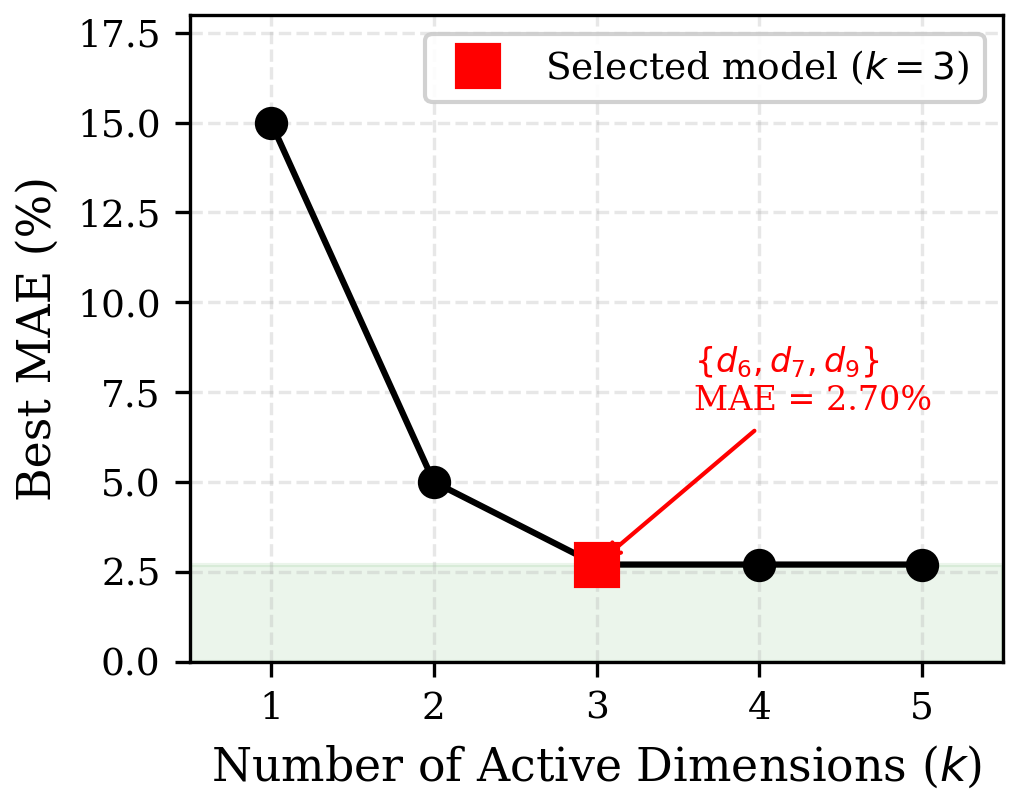
\includegraphics[width=\columnwidth]{figures/pareto.pdf}
\caption{Pareto frontier of model dimensionality against prediction error (MAE, lower is better). The elbow at $k=3$ dimensions is the selected model. Models with $k \geq 4$ add parameters without a meaningful reduction in MAE.}
\label{fig:pareto}
\end{figure}

\subsection{Sensitivity Profile}

Fig.~\ref{fig:sensitivity} shows the ablation-based sensitivity profile.
Removing epistemic status ($d_9$) causes the largest increase in MAE, consistent with its role as the highest-sensitivity dimension.
Removing social impact ($d_6$) or virtue and identity ($d_7$) also degrades performance substantially.
Removing any inactive dimension has zero effect.

\begin{figure}[!t]
\centering
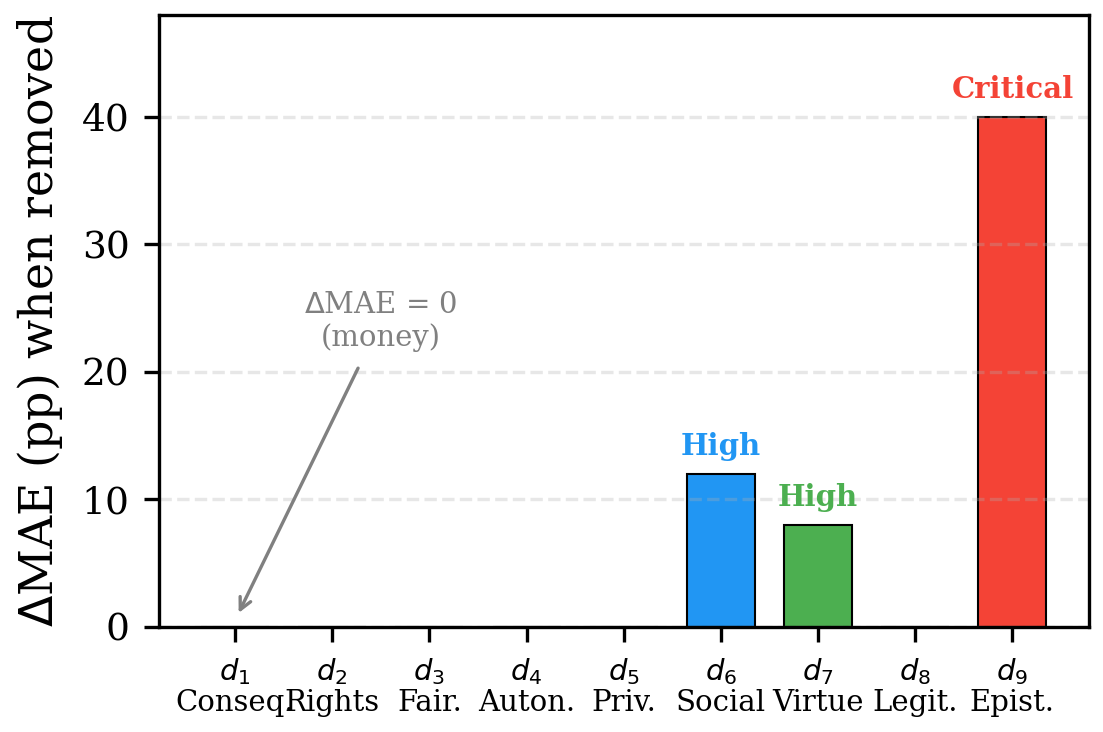
\includegraphics[width=\columnwidth]{figures/sensitivity.pdf}
\caption{Dimension sensitivity profile from ablation. Each bar shows the increase in MAE when that dimension is removed from the model, so taller is more important. Epistemic status ($d_9$) is the most sensitive dimension and the monetary dimension ($d_1$) has zero sensitivity.}
\label{fig:sensitivity}
\end{figure}

\subsection{Predicted Against Observed}

Fig.~\ref{fig:scatter} plots predicted against observed values for all sixteen targets.
Points cluster around the line of perfect prediction, with the two small-probability lotteries P16 and P17 the visible exceptions.
Game targets (circles) and lottery targets (triangles) are intermixed, so the model does not systematically over-predict or under-predict in either domain.

\begin{figure}[!t]
\centering
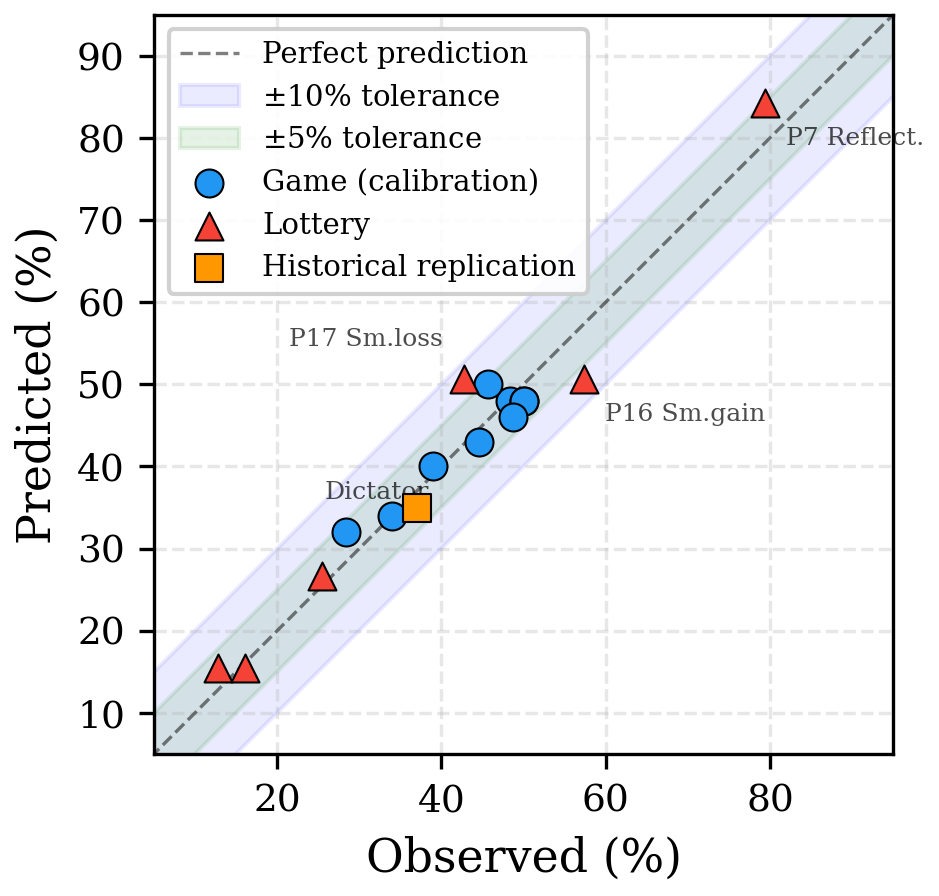
\includegraphics[width=\columnwidth]{figures/scatter.pdf}
\caption{Predicted against observed behavioral frequencies for all sixteen targets. The dashed line is perfect prediction. Circles are calibration game targets, triangles are lottery targets, and the square is the historical replication. All points fall within their stated tolerance bands. Horizontal error bars are shown only for targets where individual-level Fraser--Nettle data were recoverable.}
\label{fig:scatter}
\end{figure}


%==============================================================================
\section{Discussion}
\label{sec:discussion}
%==============================================================================

\subsection{Money-Zero as a Falsifiable Prediction}
\label{sec:andersen}

The most counterintuitive result of the calibration is that the monetary dimension ($d_1$) has exactly zero sensitivity in the selected model.
This does not mean that money is irrelevant to economic decisions.
It means that in the specific games and lotteries studied here the behavioral signal of monetary stakes is fully absorbed by the social-impact, identity, and epistemic coordinates.
In the ultimatum encoding the offer share moves the social and identity coordinates directly and moves the epistemic coordinate through rejection risk, and the selected metric recovers the observed offer from those three coordinates alone.

\subsubsection{The stake-scaling-invariance corollary}
Because $d_1$ is inactive in the selected metric, the Mahalanobis cost is invariant to any positive rescaling of the monetary coordinate.
A direct corollary is that multiplying every stake by a constant leaves the predicted offer distribution and the predicted rejection rate unchanged, conditional on offer share.
This is a sharp and falsifiable prediction.
It holds for any encoding in which the stake enters only through the monetary coordinate.
The reference implementation normalizes that coordinate to the stake, so under the present encoding the prediction would hold even at finite $\sigma_1^2$, and a rejection of invariance refutes the pair of encoding and metric together.
If observed offers or rejections vary systematically with the stake multiplier, the model as calibrated is wrong outside the calibration setting.

\subsubsection{Counterfactual activation}
Forcing $d_1$ active with $\sigma_1^2=100$, a moderate sensitivity, increases MAE from 2.70\% to 4.97\% and drops the pass count to 15/16.
At $\sigma_1^2=10$, a high sensitivity, MAE rises to 11.46\% with 7/16 passing.
The structural search therefore prefers $d_1$ inactive within the calibration setting, and the corollary is not an under-fitting artifact.

\subsubsection{Direct empirical test on high-stakes data}
We test the corollary on the high-stakes ultimatum experiment of Andersen, Erta\c{c}, Gneezy, Hoffman, and List~\cite{andersen2011}, which is to our knowledge the cleanest available test.
The experiment was run in eight villages in the state of Meghalaya in northeast India with $N=458$ responders and an equal number of proposers, at four stake levels of Rs~20, Rs~200, Rs~2{,}000, and Rs~20{,}000.
The authors report an average yearly income of about Rs~17{,}000 in the villages surveyed, so the highest stake is a little over a year's income and the Rs~2{,}000 stake is about a month and a half of income.
None of this range was used in the calibration.
We restrict to the Andersen subsample of the openICPSR replication archive~\cite{andersendata2011} and pre-specify three tests.

\textbf{Test 1 (proposer behavior).}
A Kruskal--Wallis test of equality of offer share across stake levels gives $H=60.7$ and $p=4.17\times10^{-13}$.
Invariance is rejected.
Mean offers fall monotonically from $24.2\%$ at Rs~20 to $12.1\%$ at Rs~20{,}000.

\textbf{Test 2 (responder behavior, unconditional).}
A $\chi^2$ test of independence between stake level and rejection gives $\chi^2(3,N=458)=16.18$ and $p=0.0010$.
Rejection rates fall from $36.3\%$ at Rs~20 to $4.2\%$ at Rs~20{,}000.

\textbf{Test 3 (responder behavior, conditional on offer share).}
A logit regression of rejection on offer share and $\log(\text{stake})$ is compared with a baseline that uses offer share only.
The $\log(\text{stake})$ coefficient is $-0.199$ with standard error $0.052$, an odds ratio of $0.82$ per log unit, and $p=1.5\times10^{-4}$.
The likelihood-ratio test against the offer-only model gives $p=8.77\times10^{-5}$.
AIC falls from $584.9$ to $571.5$ and BIC falls from $593.1$ to $583.8$.
Even after conditioning on the fairness signal carried by offer share, the stake level retains independent predictive power, which contradicts strict invariance.

Fig.~\ref{fig:andersen} displays observed means with 95\% confidence intervals against the flat-line prediction of stake-scaling invariance.
All three higher-stake conditions fall outside the Rs~20 confidence band, both for offers and for rejections.

\begin{figure}[!t]
\centering
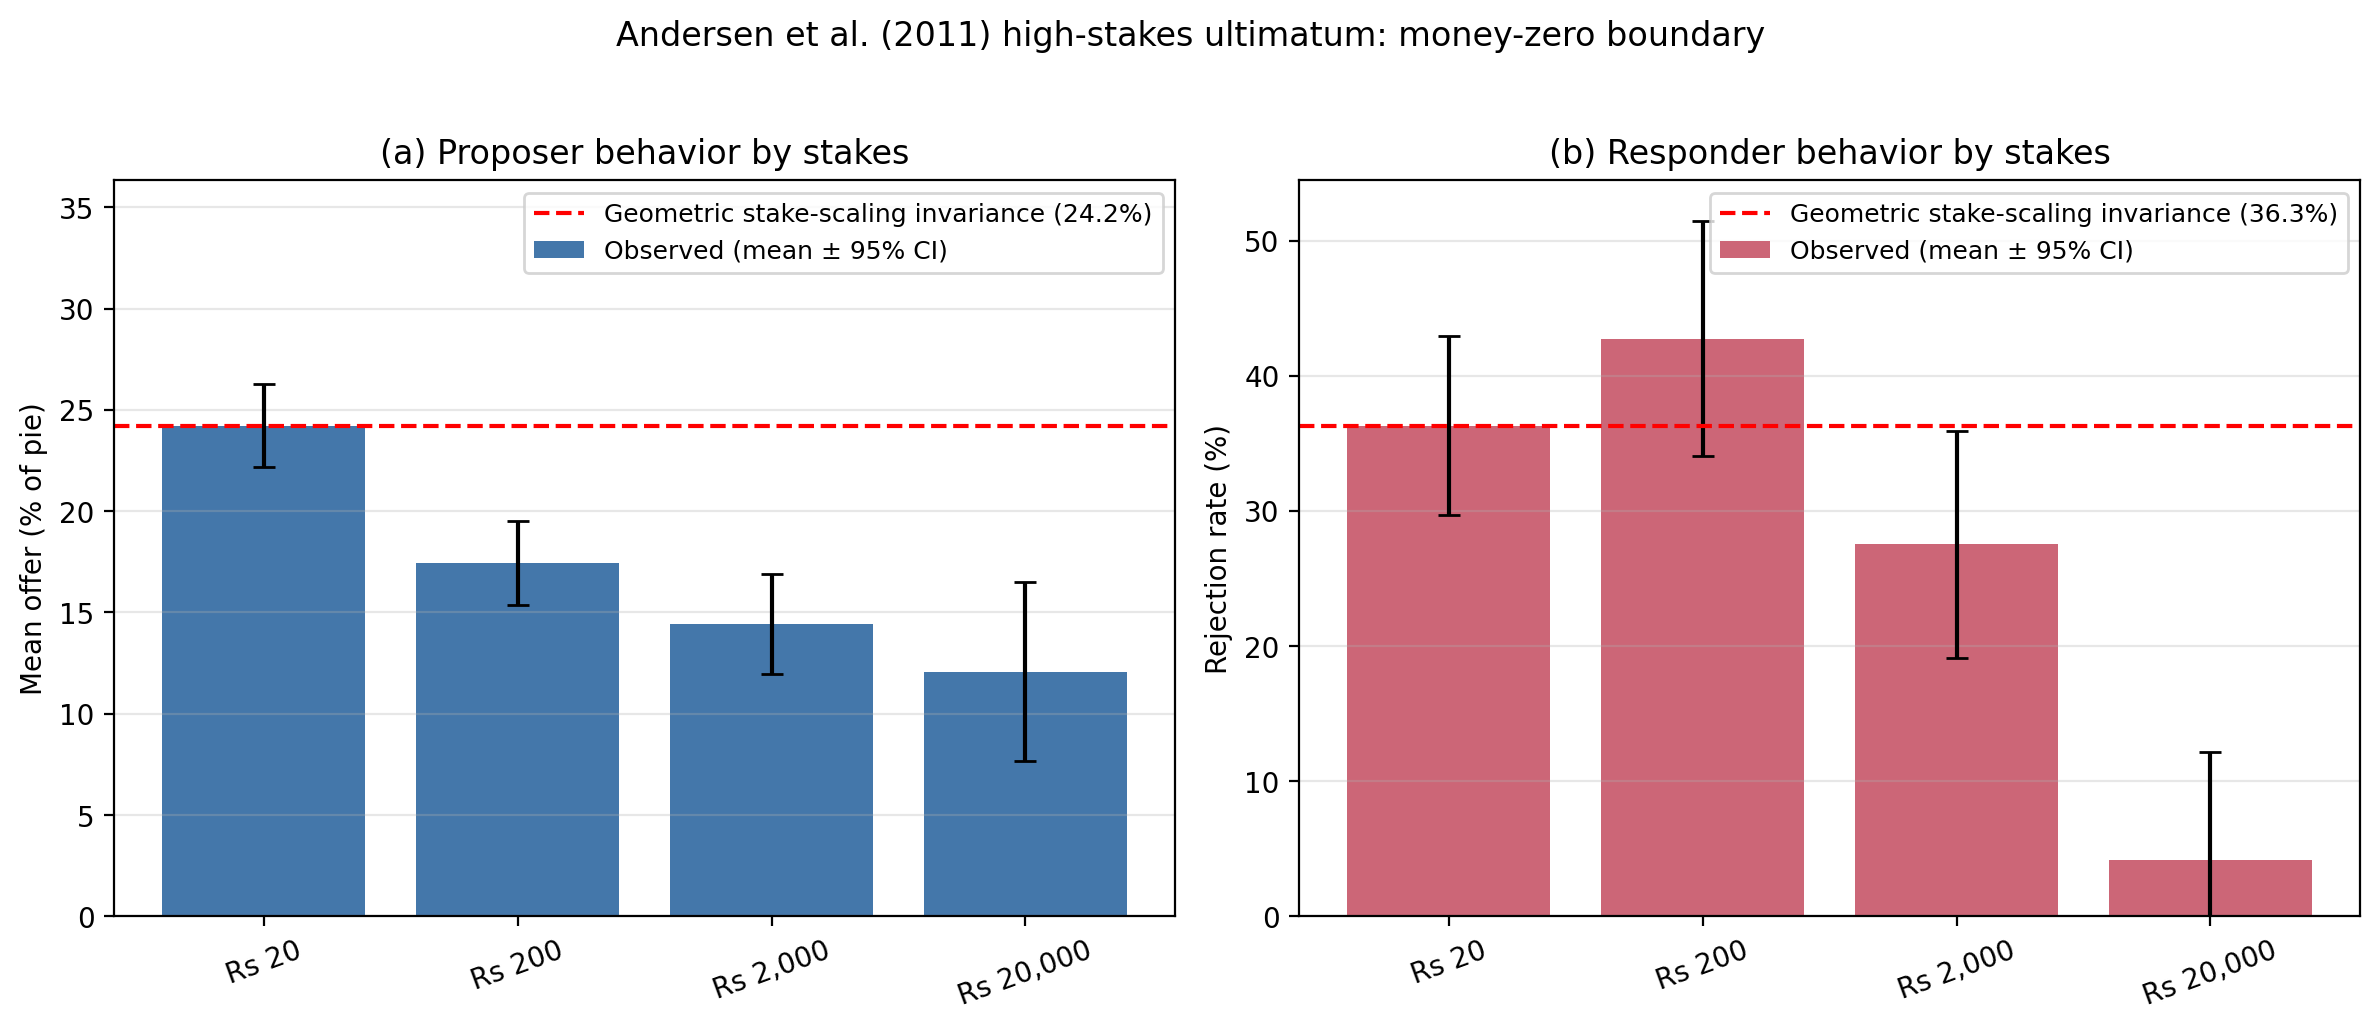
\includegraphics[width=\columnwidth]{figures/andersen_money_zero_falsification.png}
\caption{Direct test of stake-scaling invariance on the data of Andersen et al.~\cite{andersen2011} ($N=458$, Meghalaya, India). Bars show observed means with 95\% confidence intervals. The dashed line is the prediction of the calibrated share-normalized model, which is flat across stakes, anchored to the Rs~20 condition. Both panels reject invariance, with $p=4\times10^{-13}$ for offers and $p=10^{-3}$ for rejections.}
\label{fig:andersen}
\end{figure}

\subsubsection{Interpretation}
The calibrated model predicts invariance, and that prediction fails.
The model does not predict the observed direction or magnitude of the stake effect, because under the share-normalized encoding no value of the monetary variance would.
The selected metric remains a parsimonious descriptive model of the low-stakes tasks on which it was calibrated.
It does not extend unchanged to consequential-stake settings, and the universal money-zero claim is empirically false.

A model that fits both stake ranges would need a monetary coordinate in absolute or income units, so that the stake changes the displacement, together with a finite $\sigma_1^2$.
One concrete form replaces the share-normalized coordinate of Table~\ref{tab:encodings} by an income-scaled one.
With stake $\Lambda$ and a local income scale $Y$, the proposer's monetary coordinate becomes $s_1(x)=(\Lambda/Y)\,q(x)(1-x)$ with reference $r_1=\Lambda/Y$, so that the monetary displacement $\Delta a_1=(\Lambda/Y)\bigl(q(x)(1-x)-1\bigr)$ grows with the stake while every other coordinate is unchanged.
With finite $\sigma_1^2$ the monetary term $(\Lambda/Y)^2\bigl(1-q(x)(1-x)\bigr)^2/\sigma_1^2$ then penalizes generous offers more at higher stakes and moves the cost minimizer toward lower offers, which is the direction of the Andersen data, where mean offers fall from 24 percent to 12 percent across the stake range.
That form also replaces the invariance corollary by a testable one, namely that predictions depend on the stake only through the ratio $\Lambda/Y$, so two populations facing the same fraction of yearly income should show the same offers.
That model has not been fitted or tested here, and the Andersen result motivates it without testing it.
Locating the stake level at which invariance fails, and how that level depends on local income and anonymity, is a natural target for follow-up work using individual-level data from Andersen et al., Slonim and Roth~\cite{slonim1998}, Cameron~\cite{cameron1999}, and competitive double-auction settings~\cite{smith1962}.

\subsubsection{What this does not establish}
The Andersen data are one dataset from one region of one country.
The test rejects the universal money-zero claim.
It does not by itself establish where the boundary sits, how it depends on cultural or institutional context, or whether the same recalibration mechanism explains analogous boundaries in dictator and public-goods games.
Camerer's review~\cite{camerer2003} of cross-stakes ultimatum results is mixed in this respect, since stake-size invariance holds in many ranges but not in extreme conditions.
The present test demonstrates a failure of invariance and does not locate its boundary.

\subsection{A Cross-Domain Bridge, Not a Unification}

The central methodological contribution is cross-domain parameter reuse.
A metric fitted on game-theory data, meaning strategic interaction with real money, organizes six classic prospect-theory phenomena, meaning hypothetical lottery choices, within an active-set structure selected on both, and a corollary of that metric is then tested on a high-stakes ultimatum dataset that played no role in any fitting or selection step.

We do not describe this result as a unification of the two literatures.
Game theory and prospect theory are both wider than the present targets.
What the evidence supports is narrower.
A shared metric primitive is sufficient to organize a small set of canonical aggregate frequencies from both domains, conditional on explicit and auditable domain-specific encodings.
Domain-general modeling moves through the metric, which is the same $\Sigma$ in every task.
Domain-specific structure moves through the encoding layer, which maps each scenario to a reference point and a set of alternatives.
The testable content of the model is the conjunction of both.
The result is most fairly characterized as a parsimonious geometric reduction of two literatures' canonical findings to a common cost structure, rather than as a derivation of either literature from first principles.

The certainty effect in prospect theory and the rejection of unfair offers in the ultimatum game look very different at the surface, but the fitted metric routes both through high sensitivity to epistemic status ($d_9$).
A certain outcome has zero epistemic displacement from the lottery reference, and an offer likely to be accepted has zero epistemic displacement from the proposer reference.
This is an interpretive bridge, not a theorem about either literature.

The natural extension is to test the same bridge in additional domains by fitting $\Sigma$ on data from one domain and predicting behavior in others.
The present paper takes the first such step, from games to lotteries, and demonstrates one setting in which the encoding and metric must change, since stake invariance fails at consequential stakes.

\subsubsection*{Toward a tractable equilibrium model}
The emphasis on metric decision spaces also bears on the computation of equilibria.
Nash equilibrium is a consistency condition on strategy profiles and does not assume that agents compute it, but Nash equilibria exist in finite games~\cite{nash1950} while computing one is PPAD-complete~\cite{daskalakis2009,chen2009}, so any procedure that reaches equilibrium play in a large game must do so without exhaustive search.
The A$^{*}$ algorithm~\cite{hart1968} reaches an optimal path under an admissible heuristic with complete search, and truncating that search trades the optimality guarantee for tractability.
A decision space with an interpretable cost metric is one candidate space on which such a truncated search could be specified, with the interpretable dimensions as candidate heuristic coordinates.
Nothing in the present paper tests that reading, and developing it is beyond the scope of this empirical work.

\subsection{Complexity, Degrees of Freedom, and Multiplicity}

The narrow covariance-parameter count is three active variances for sixteen aggregate targets, a descriptive ratio of $16/3=5.3$.
This number should not be read as the complete complexity of the modeling exercise.
As Table~\ref{tab:param_accounting} shows, the temperature, the rejection function, the public-goods drift, the certainty operator, the domain-dependent coding, the epistemic reference values, the diagonal restriction, and the nine-dimensional basis all contribute flexibility or structure.

A conservative count that includes the three active variances, two temperature constants, one temperature floor, two rejection-function constants, two drift constants, and three lottery encoding mechanisms yields thirteen named quantities, before counting the coordinate constants of Table~\ref{tab:encodings} and the basis itself.
This does not make the model uninformative.
It does mean that the parsimony claim should be read as ``few fitted covariance variances conditional on an explicit encoding architecture,'' not as ``only three choices were made.''

The structural search also creates multiplicity exposure, since 381 active-set structures are considered before $\{d_6,d_7,d_9\}$ is selected, and the ranking among them used all sixteen targets.
Because the objective is deterministic aggregate prediction error rather than a set of independent null-hypothesis tests, Bonferroni-style $p$ values are not directly applicable.
The appropriate interpretation is model selection.
We report the search exposure and rely on the fitting accounting of Section~\ref{sec:heldout}, the ablations, and the independent Andersen probe rather than on significance language.

\subsection{What the Result Is, and Is Not, About Rationality}
\label{sec:not-rationality}

It is tempting to frame the result as showing that behavioral anomalies are rational navigation on a manifold.
The empirical exercise does not support that reading.
What it shows is much narrower.
A particular encoding-and-metric system reproduces a small set of canonical aggregate frequencies from two literatures with three fitted variances, conditional on the encodings, and the model's stake-invariance corollary fails when probed outside its calibration setting.
None of that establishes that the underlying behavior is rational in a normative sense, that agents optimize the geometric cost, or that the dimensions correspond to psychological primitives.

We therefore use \emph{descriptive geometric reduction} as the operative description of the result.
The model is descriptive in the sense that $\Sigma$ summarizes observed choice frequencies.
It is geometric in the sense that the cost structure is a metric on a vector space rather than a scalar utility.
It is a reduction in the sense that two literatures' canonical findings are organized through a common nine-dimensional vocabulary.
Whether this reduction corresponds to anything that could be called rationality is left open.

\subsection{Normative Labels, Descriptive Use}
\label{sec:descriptive-labels}

The dimension names fairness, virtue and identity, legitimacy, and epistemic status are ordinarily normative.
They are used here as descriptive coordinate labels chosen for interpretability, not as normative endorsements.
What the calibration constrains is the geometry of $\Sigma$.
A variance is small when small displacement on that coordinate produces large changes in observed choice frequencies, regardless of whether the coordinate would be considered normatively weighty or psychologically primitive.
The labels let a reader connect the metric structure to existing literatures, Fehr--Schmidt on fairness, Haidt on identity, Ellsberg on ambiguity.
They are not a claim that the model has measured those constructs.
A model with identical metric behavior but neutral coordinate labels $(z_1,\dots,z_9)$ would make the same predictions.

For the same reason we do not claim that the present nine-dimensional basis is uniquely correct or psychometrically derived.
The basis is a modeling vocabulary that spans material, procedural, social, and epistemic content (Table~\ref{tab:dimensions}).
A derived basis would require individual-level multi-task data and dimensional-reduction techniques that the present aggregate benchmark does not support.
Future work should compare the present labels against alternative bases, such as factor-analytic decompositions of multi-task individual-level choices, automated text-to-attribute encoders, or expert-rated coordinate sets, to test whether the metric result survives a change of basis.

\subsection{Implications for Computational Social Systems}

The geometric model has four implications for computational social systems.
\begin{enumerate}
    \item \textbf{Agent modeling}. Computational agents in social simulations can be endowed with a Mahalanobis cost function on nine dimensions, producing more realistic behavior than scalar utility maximizers.
    \item \textbf{Policy simulation}. Policy interventions that change the encoding, for example framing a tax as a contribution to the common good, which shifts $d_6$ and $d_7$, can be modeled as changes in the displacement vector, with behavioral consequences predicted by the cost metric.
    \item \textbf{Mechanism design}. Mechanism designers should attend to all nine dimensions, not only monetary incentives. A mechanism that is optimal on $d_1$ but costly on $d_7$, for example because it requires participants to behave in ways that conflict with their self-image, may fail in practice.
    \item \textbf{Cultural variation}. Cross-cultural differences in economic behavior~\cite{henrich2010} may be modeled as differences in $\Sigma$, meaning that cultures weight the nine dimensions differently, rather than as differences in rationality.
\end{enumerate}

\subsection{Minimal Agent-Based Worked Example}

To make the computational-social-systems use case concrete, Fig.~\ref{fig:abm} gives a minimal agent-based illustration.
This is not an additional empirical validation.
It shows how the fitted covariance can be used as an agent behavioral primitive.
Each geometric agent draws a small perturbation around the active variances and chooses an ultimatum offer by the softmax rule over candidate offers.
A scalar expected-value agent places offers near zero, while a simple Fehr--Schmidt-like heterogeneous population produces a broader inequality-aversion distribution.
Under the calibrated variances the cost differences between offers are small relative to the softmax temperature, so the geometric agents spread their offers almost uniformly between zero and the equal split. The figure illustrates that a named metric can be used as a behavioral primitive in a simulation, not that this minimal setup reproduces an observed offer distribution.

\begin{figure}[!t]
\centering
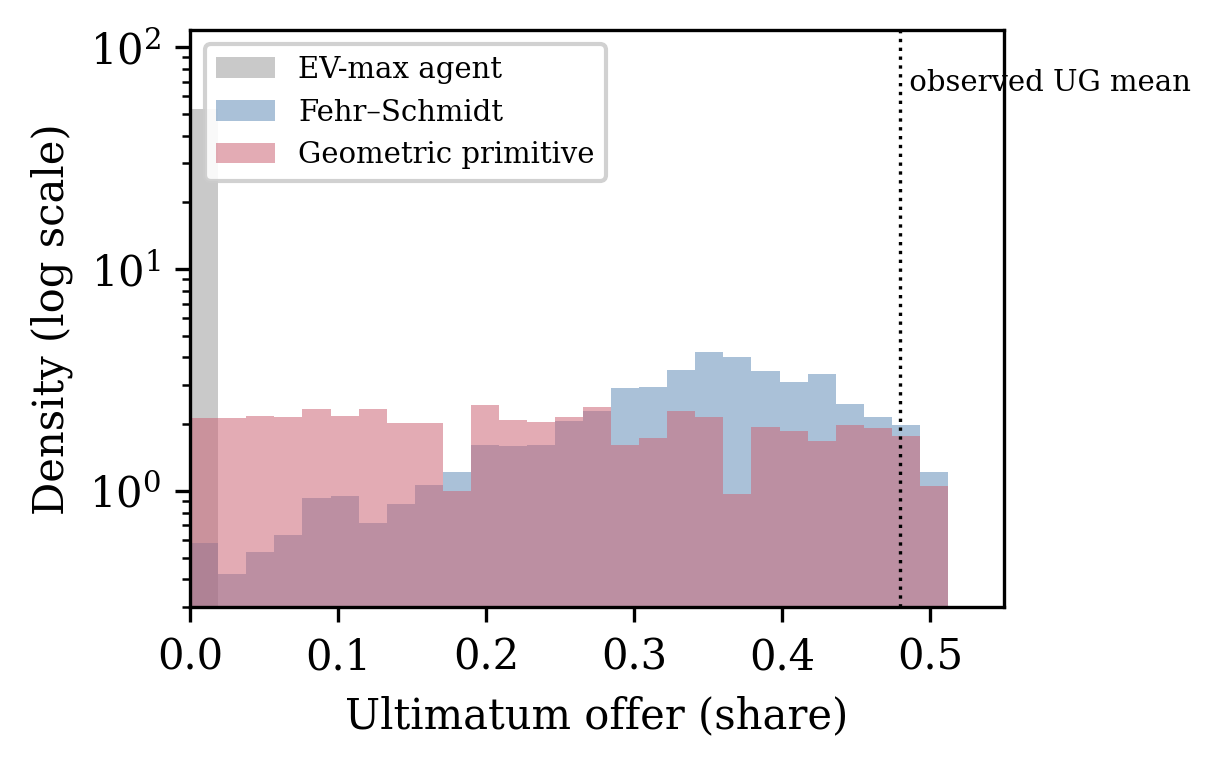
\includegraphics[width=\columnwidth]{figures/abm_worked_example.pdf}
\caption{Minimal agent-based illustration using the geometric metric as a behavioral primitive. The geometric agents spread offers almost uniformly from zero to the equal split, the expected-value agents offer near zero, and the inequality-averse population peaks near a 35 percent offer. The figure is illustrative and is not a new validation experiment.}
\label{fig:abm}
\end{figure}

\subsection{Limitations}

Nine limitations qualify the present results.
\begin{enumerate}
    \item \textbf{Encoding dependence}. The benchmark validates the metric conditional on researcher-coded encodings. The certainty operator, the domain-dependent coding, the epistemic reference values, and the coordinate constants of Table~\ref{tab:encodings} are fixed assumptions tested by ablation, not independently established psychological laws. External raters, preregistered coding rules, or automated scenario-to-attribute encoders are needed to separate encoding validation from metric validation.
    \item \textbf{Narrow target battery}. The lottery set contains six classic targets, the historical replication target is a single 1982 ultimatum result, and the high-stakes boundary test uses one dataset from northeast India. The 19-country replication of Ruggeri et al.~\cite{ruggeri2020}, additional high-stakes bargaining cohorts (Slonim and Roth~\cite{slonim1998}, Cameron~\cite{cameron1999}), non-WEIRD samples, trust games, and market-exchange datasets are necessary before broad claims can be made.
    \item \textbf{Aggregate data on the calibration side}. Most calibration targets are published summaries from heterogeneous studies rather than a single individual-level dataset. This prevents joint likelihood estimation across the full benchmark. The Andersen boundary test performs the falsification probe on individual-level data, but the calibration itself remains aggregate.
    \item \textbf{Tolerance-based evaluation}. The 16/16 pass rate is an engineering diagnostic. The MAE on the high-$N$ Ruggeri lottery subset is 3.95\%, against 2.70\% averaged over the full benchmark, and two lottery predictions (P16, P17) fall outside the Ruggeri 95\% interval despite passing the $\pm10$~pp tolerance. Future work should adopt common train, validation, and test splits with individual-level likelihoods throughout.
    \item \textbf{No fully out-of-sample lottery target}. The temperature constants were set from P1 and P3, the G\"uth reference coordinate was set from the G\"uth offer, and the ranking of active sets used all sixteen targets, so the lottery results demonstrate parameter reuse within a jointly selected architecture rather than out-of-sample prediction. The temperature rule is nonmonotone above a cost gap of $1.41$, where four of the six lottery targets lie, and the ordering of P1 against P3 is carried by that rule rather than by the geometry (Section~\ref{sec:framework}).
    \item \textbf{Model complexity}. The three-parameter description counts only active covariance variances. A fuller accounting includes the temperature, rejection, drift, and encoding mechanisms and the structural restrictions. The conservative count is thirteen named quantities (Table~\ref{tab:param_accounting}) plus the coordinate constants.
    \item \textbf{Diagonal covariance}. The diagonal model cannot represent interactions such as fairness-by-social-impact coupling or epistemic-status modulation of identity. Full or sparse covariance estimation requires more observations than the present aggregate benchmark provides. We treat this as a deferred extension rather than a closed question.
    \item \textbf{Failure of invariance demonstrated, boundary not located}. The Andersen test rejects the calibrated model's stake-scaling invariance but does not locate the stake at which it fails, does not test a monetary coordinate in absolute or income units, and does not map the failure across cultures, institutional settings, or game types.
    \item \textbf{Static and mostly binary choices}. The softmax rule handles binary choices, and the game predictions are deterministic cost minima over static menus. Multi-alternative stochastic choice, learning, belief updating, and repeated strategic adaptation remain extensions. The agent-based example is illustrative, and full mechanism-design and policy-simulation applications are not implemented here.
\end{enumerate}

%==============================================================================
\section{Conclusion}
\label{sec:conclusion}
%==============================================================================

This paper presents and tests a geometric model of economic behavior in which decisions are displacements from a task reference point in a nine-dimensional space and are evaluated by Mahalanobis cost.
A diagonal covariance fitted on game-theoretic aggregate targets matches a small set of lottery and historical-replication targets without refitting the active variances, within an active-set structure that was selected on the full benchmark.
The selected active set, social impact, virtue and identity, and epistemic status, identifies the dominant metric dimensions in this benchmark, and the monetary dimension is inactive in the selected metric.

The model's most counterintuitive prediction, stake-scaling invariance, is tested on the high-stakes ultimatum data of Andersen et al.~\cite{andersen2011} from Meghalaya, India ($N=458$, a thousandfold stake range), and all three pre-specified tests reject it.
The calibrated model predicts invariance and that prediction fails, so the share-normalized encoding and the selected metric do not extend unchanged to consequential stakes.
The result motivates, but does not test, a monetary coordinate in absolute or income units with finite sensitivity.

The main contribution is not a unification of behavioral economics.
It is a self-contained, interpretable, and falsifiable cross-domain modeling architecture, specified down to every coded constant, accompanied by a direct test of its strongest counterintuitive prediction.
The model can be embedded in computational social-system simulations as an interpretable behavioral primitive.
Its broader validity depends on stronger tests still to come, namely individual-level joint estimation across the full benchmark, multi-country lottery replications under a common protocol, additional high-stakes bargaining cohorts with an income-scaled monetary coordinate to locate the stake at which invariance fails, market-exchange data, non-diagonal covariance structures, and preregistered encoding rules with external raters.

\section*{Acknowledgment}
Generative AI tools (Claude, Anthropic) were used to assist with manuscript drafting, editing, formatting, and code review.
The research questions, model, experimental design, analyses, and conclusions are the author's own, and the author verified every reported number against the released reference implementation and the cited public datasets.

\appendices
\section{CPT Baseline: Per-Target Errors}
\label{app:cpt}

Table~\ref{tab:cpt_detail} reports CPT predictions for each lottery target under the canonical parameters from Tversky and Kahneman~\cite{tversky1992}.
All six absolute errors are below the $\pm10$~pp criterion, so canonical CPT passes 6/6 with MAE 5.7\%.
No refitted CPT is reported.

\begin{table}[!h]
\renewcommand{\arraystretch}{1.15}
\caption{CPT Per-Target Errors Under the Canonical Parameters}
\label{tab:cpt_detail}
\centering
\begin{tabular}{l r r r c}
\toprule
\textbf{Target} & \textbf{Obs.} & \textbf{Pred.} & \textbf{Err.} & \textbf{Pass} \\
\midrule
P1 Allais       & 25.5\% & 30.2\% & +4.7   & \checkmark \\
P3 Strong cert.  & 12.8\% & 20.4\% & +7.6   & \checkmark \\
P7 Reflection   & 79.4\% & 74.1\% & $-$5.3 & \checkmark \\
P11 Isolation   & 16.1\% & 20.4\% & +4.3   & \checkmark \\
P16 Sm.\ gain   & 57.4\% & 60.8\% & +3.4   & \checkmark \\
P17 Sm.\ loss   & 42.8\% & 51.6\% & +8.8   & \checkmark \\
\midrule
\textbf{MAE}    &        & \multicolumn{2}{c}{\textbf{5.7\%}} & \textbf{6/6} \\
\bottomrule
\end{tabular}
\begin{flushleft}
\footnotesize{Canonical parameters are $\alpha=0.88$, $\beta=0.88$, $\lambda=2.25$, $\gamma=0.61$, $\delta=0.69$.
The pass criterion is $|\text{Error}| \leq 10$~pp.
P11 is evaluated in its reduced form, so its canonical prediction equals that of P3.}
\end{flushleft}
\end{table}

%==============================================================================
% References
%==============================================================================

\begin{thebibliography}{45}

\bibitem{vonneumann1944}
J.~von Neumann and O.~Morgenstern, \emph{Theory of Games and Economic Behavior}.
Princeton, NJ, USA: Princeton Univ. Press, 1944.
\bibitem{savage1954}
L.~J.~Savage, \emph{The Foundations of Statistics}.
New York, NY, USA: Wiley, 1954.
\bibitem{kahneman1979}
D.~Kahneman and A.~Tversky, ``Prospect theory: An analysis of decision under risk,''
\emph{Econometrica}, vol.~47, no.~2, pp.~263--291, Mar. 1979.
\bibitem{tversky1992}
A.~Tversky and D.~Kahneman, ``Advances in prospect theory: Cumulative representation of uncertainty,''
\emph{J. Risk Uncertainty}, vol.~5, no.~4, pp.~297--323, Oct. 1992, doi: 10.1007/BF00122574.
\bibitem{fehr1999}
E.~Fehr and K.~M.~Schmidt, ``A theory of fairness, competition, and cooperation,''
\emph{Quart. J. Econ.}, vol.~114, no.~3, pp.~817--868, Aug. 1999, doi: 10.1162/003355399556151.
\bibitem{bolton2000}
G.~E.~Bolton and A.~Ockenfels, ``ERC: A theory of equity, reciprocity, and competition,''
\emph{Amer. Econ. Rev.}, vol.~90, no.~1, pp.~166--193, Mar. 2000, doi: 10.1257/aer.90.1.166.
\bibitem{ruggeri2020}
K.~Ruggeri \emph{et~al.}, ``Replicating patterns of prospect theory for decision under risk,''
\emph{Nature Human Behav.}, vol.~4, no.~6, pp.~622--633, Jun. 2020, doi: 10.1038/s41562-020-0886-x.
\bibitem{henrich2010}
J.~Henrich, S.~J.~Heine, and A.~Norenzayan, ``The weirdest people in the world?''
\emph{Behav. Brain Sci.}, vol.~33, no.~2--3, pp.~61--83, Jun. 2010, doi: 10.1017/S0140525X0999152X.
\bibitem{andersen2011}
S.~Andersen, S.~Erta\c{c}, U.~Gneezy, M.~Hoffman, and J.~A.~List, ``Stakes matter in ultimatum games,''
\emph{Amer. Econ. Rev.}, vol.~101, no.~7, pp.~3427--3439, Dec. 2011, doi: 10.1257/aer.101.7.3427.
\bibitem{keeney1993}
R.~L.~Keeney and H.~Raiffa, \emph{Decisions with Multiple Objectives: Preferences and Value Trade-Offs}.
Cambridge, U.K.: Cambridge Univ. Press, 1993.
\bibitem{cheng2026urban}
L.~Cheng, M.~Li, C.~Tan, P.~Huang, M.~Zhang, and R.~Sun, ``Computational game-theoretic models for adaptive urban energy systems: A comprehensive review of algorithms, strategies, and engineering applications,''
\emph{Arch. Comput. Methods Eng.}, vol.~33, no.~2, pp.~2037--2114, Mar. 2026, doi: 10.1007/s11831-025-10364-y.
\bibitem{cheng2025vpp}
L.~Cheng, M.~Zhang, K.~Wang, M.~Yuan, Z.~Liu, J.~Wang, K.~Zhang, and P.~Huang, ``Evolutionary smart contracts for virtual power plant trading: Integrating prospect theory and multi-stage negotiation in cross-regional energy markets,''
\emph{Int. J. Elect. Power Energy Syst.}, vol.~173, Art.~no.~111453, Dec. 2025, doi: 10.1016/j.ijepes.2025.111453.
\bibitem{train2009}
K.~E.~Train, \emph{Discrete Choice Methods with Simulation}, 2nd~ed.
Cambridge, U.K.: Cambridge Univ. Press, 2009.
\bibitem{hastie2009}
T.~Hastie, R.~Tibshirani, and J.~Friedman, \emph{The Elements of Statistical Learning}, 2nd~ed.
New York, NY, USA: Springer, 2009.
\bibitem{smith1962}
V.~L.~Smith, ``An experimental study of competitive market behavior,''
\emph{J. Polit. Econ.}, vol.~70, no.~2, pp.~111--137, Apr. 1962.
\bibitem{arrow1951}
K.~J.~Arrow, \emph{Social Choice and Individual Values}.
New York, NY, USA: Wiley, 1951.
\bibitem{ostrom1990}
E.~Ostrom, \emph{Governing the Commons: The Evolution of Institutions for Collective Action}.
Cambridge, U.K.: Cambridge Univ. Press, 1990.
\bibitem{sen1999}
A.~Sen, \emph{Development as Freedom}.
New York, NY, USA: Knopf, 1999.
\bibitem{akerlof1970}
G.~A.~Akerlof, ``The market for `lemons': Quality uncertainty and the market mechanism,''
\emph{Quart. J. Econ.}, vol.~84, no.~3, pp.~488--500, Aug. 1970.
\bibitem{stiglitz1981}
J.~E.~Stiglitz and A.~Weiss, ``Credit rationing in markets with imperfect information,''
\emph{Amer. Econ. Rev.}, vol.~71, no.~3, pp.~393--410, Jun. 1981.
\bibitem{camerer2003}
C.~F.~Camerer, \emph{Behavioral Game Theory: Experiments in Strategic Interaction}.
Princeton, NJ, USA: Princeton Univ. Press, 2003.
\bibitem{haidt2012}
J.~Haidt, \emph{The Righteous Mind: Why Good People Are Divided by Politics and Religion}.
New York, NY, USA: Vintage Books, 2012.
\bibitem{tetlock2000}
P.~E.~Tetlock, ``Coping with trade-offs: Psychological constraints and political implications,''
in \emph{Elements of Reason: Cognition, Choice, and the Bounds of Rationality},
A.~Lupia, M.~D.~McCubbins, and S.~L.~Popkin, Eds.
Cambridge, U.K.: Cambridge Univ. Press, 2000, pp.~239--263.
\bibitem{thaler2008}
R.~H.~Thaler and C.~R.~Sunstein, \emph{Nudge: Improving Decisions About Health, Wealth, and Happiness}.
New Haven, CT, USA: Yale Univ. Press, 2008.
\bibitem{simon1955}
H.~A.~Simon, ``A behavioral model of rational choice,''
\emph{Quart. J. Econ.}, vol.~69, no.~1, pp.~99--118, Feb. 1955.
\bibitem{ellsberg1961}
D.~Ellsberg, ``Risk, ambiguity, and the Savage axioms,''
\emph{Quart. J. Econ.}, vol.~75, no.~4, pp.~643--669, Nov. 1961.
\bibitem{mahalanobis1936}
P.~C.~Mahalanobis, ``On the generalised distance in statistics,''
\emph{Proc. Nat. Inst. Sci. India}, vol.~2, no.~1, pp.~49--55, Apr. 1936.
\bibitem{eriseconsw}
A.~H.~Bond, ``eris-econ: Geometric economics on multi-dimensional decision manifolds,'' ver.~0.1.0, Zenodo, Jun. 2026, doi: 10.5281/zenodo.20660123. [Online]. Available: \url{https://pypi.org/project/eris-econ/}
\bibitem{engel2011}
C.~Engel, ``Dictator games: A meta study,''
\emph{Exp. Econ.}, vol.~14, no.~4, pp.~583--610, Nov. 2011, doi: 10.1007/s10683-011-9283-7.
\bibitem{fraser2020}
S.~Fraser and D.~Nettle, ``Hunger affects social decisions in a multi-round public goods game but not a single-shot ultimatum game,''
\emph{Adaptive Human Behav. Physiol.}, vol.~6, no.~3, pp.~334--355, Sep. 2020, doi: 10.1007/s40750-020-00143-3.
\bibitem{allais1953}
M.~Allais, ``Le comportement de l'homme rationnel devant le risque: Critique des postulats et axiomes de l'\'{e}cole Am\'{e}ricaine,''
\emph{Econometrica}, vol.~21, no.~4, pp.~503--546, Oct. 1953.
\bibitem{guth1982}
W.~G\"{u}th, R.~Schmittberger, and B.~Schwarze, ``An experimental analysis of ultimatum bargaining,''
\emph{J. Econ. Behav. Org.}, vol.~3, no.~4, pp.~367--388, Dec. 1982, doi: 10.1016/0167-2681(82)90011-7.
\bibitem{fraserdata2020}
S.~Fraser and D.~Nettle, ``Data and code for Fraser and Nettle, `Hunger affects social decisions in a public goods game but not an ultimatum game','' Zenodo, ver.~3, 2020, doi: 10.5281/zenodo.3764693.
\bibitem{andersendata2011}
S.~Andersen, S.~Erta\c{c}, U.~Gneezy, M.~Hoffman, and J.~A.~List, ``Replication data for: Stakes matter in ultimatum games,''
American Economic Association/openICPSR study 112485, 2019, doi: 10.3886/E112485V1.
\bibitem{slonim1998}
R.~Slonim and A.~E.~Roth, ``Learning in high stakes ultimatum games: An experiment in the Slovak Republic,''
\emph{Econometrica}, vol.~66, no.~3, pp.~569--596, May 1998, doi: 10.2307/2998575.
\bibitem{cameron1999}
L.~A.~Cameron, ``Raising the stakes in the ultimatum game: Experimental evidence from Indonesia,''
\emph{Econ. Inquiry}, vol.~37, no.~1, pp.~47--59, Jan. 1999, doi: 10.1111/j.1465-7295.1999.tb01415.x.
\bibitem{nash1950}
J.~F.~Nash, ``Equilibrium points in $n$-person games,''
\emph{Proc. Nat. Acad. Sci. USA}, vol.~36, no.~1, pp.~48--49, Jan. 1950.
\bibitem{daskalakis2009}
C.~Daskalakis, P.~W.~Goldberg, and C.~H.~Papadimitriou, ``The complexity of computing a Nash equilibrium,''
\emph{SIAM J. Comput.}, vol.~39, no.~1, pp.~195--259, 2009, doi: 10.1137/070699652.
\bibitem{chen2009}
X.~Chen, X.~Deng, and S.-H.~Teng, ``Settling the complexity of computing two-player Nash equilibria,''
\emph{J. ACM}, vol.~56, no.~3, Art.~no.~14, May 2009, doi: 10.1145/1516512.1516516.
\bibitem{hart1968}
P.~E.~Hart, N.~J.~Nilsson, and B.~Raphael, ``A formal basis for the heuristic determination of minimum cost paths,''
\emph{IEEE Trans. Syst. Sci. Cybern.}, vol.~4, no.~2, pp.~100--107, Jul. 1968.
\end{thebibliography}

\begin{IEEEbiographynophoto}{Andrew H. Bond}
received the B.S.E.E. degree from North Carolina State University and the M.S.S.E. degree from San Jos\'{e} State University. He has over 20 years of industry experience at AT\&T, Cisco Systems, and Fujitsu Network Communications. He is currently with the Department of Computer Engineering, San Jos\'{e} State University, San Jos\'{e}, CA, USA, where he teaches and advises graduate theses. His research interests include computational models of social and economic behavior, embedding compression, autonomous security agents, and cognitive architectures. He is a Senior Member of IEEE.
\end{IEEEbiographynophoto}

\balance

\end{document}
